\documentclass[aspectratio=169,11pt]{beamer}
\usepackage[utf8]{inputenc}
\usepackage[T1]{fontenc}
\usepackage[polish]{babel}
\usepackage{graphicx}
\usepackage{booktabs}
\usepackage{tikz}
\usepackage{listings}
\usepackage{xcolor}
\usepackage{hyperref}
\usepackage{array}
\usepackage{colortbl}
\usepackage{amsmath}
\usepackage{amssymb}

\hypersetup{
    colorlinks=true,
    linkcolor=blue,
    filecolor=magenta,      
    urlcolor=cyan,
    pdftitle={Overleaf Example},
    pdfpagemode=FullScreen,
    }

\urlstyle{same}

% Ścieżka do obrazków
\graphicspath{{./img/}{./}}

% Konfiguracja kolorów
\definecolor{yoloBlue}{RGB}{30,60,114}
\definecolor{yoloPurple}{RGB}{100,80,180}
\definecolor{codeBackground}{RGB}{40,44,52}
\definecolor{codeText}{RGB}{171,178,191}
\definecolor{codeKeyword}{RGB}{198,120,221}
\definecolor{codeString}{RGB}{152,195,121}
\definecolor{codeComment}{RGB}{92,99,112}
\definecolor{darkgreen}{RGB}{0,128,0}

% Motyw prezentacji
\usetheme{Madrid}
\usecolortheme{whale}
\setbeamercolor{structure}{fg=yoloBlue}
\setbeamercolor{title}{fg=white,bg=yoloBlue}
\setbeamercolor{frametitle}{fg=white,bg=yoloBlue}

% Konfiguracja listings dla kodu
\lstset{
    backgroundcolor=\color{codeBackground},
    basicstyle=\ttfamily\small\color{codeText},
    keywordstyle=\color{codeKeyword},
    stringstyle=\color{codeString},
    commentstyle=\color{codeComment},
    breaklines=true,
    showstringspaces=false,
    frame=single,
    rulecolor=\color{codeBackground}
}

\title{\textbf{YOLO}}
\subtitle{Detekcja obiektów w czasie rzeczywistym}
\author{Warsztat praktyczny}
\date{}

\begin{document}

% =============================================================================
% SLAJD TYTUŁOWY
% =============================================================================
\begin{frame}
\titlepage
\end{frame}

% =============================================================================
% CZĘŚĆ 1: WPROWADZENIE I KONTEKST
% =============================================================================
\section{Wprowadzenie i kontekst}

% -----------------------------------------------------------------------------
% Slajd: Agenda części 1
% -----------------------------------------------------------------------------
\begin{frame}{Część 1: Wprowadzenie i kontekst}
\tableofcontents[currentsection]
\begin{itemize}
    \item Czym jest detekcja obiektów vs klasyfikacja vs segmentacja
    \item Historia: od R-CNN do YOLO
    \item Filozofia YOLO: ``You Only Look Once''
    \item Ewolucja wersji YOLO
    \item Którą wersję wybrać i dlaczego
\end{itemize}
\end{frame}

% -----------------------------------------------------------------------------
% Slajd: Klasyfikacja obrazów
% -----------------------------------------------------------------------------
\begin{frame}{Klasyfikacja obrazów}
\begin{columns}
\begin{column}{0.6\textwidth}
\textbf{Klasyfikacja -- CO to jest?}
\begin{itemize}
    \item Przypisanie \textbf{jednej etykiety} do całego obrazu
    \item Wyjście: etykieta + prawdopodobieństwo
    \item Przykład: ``kot'' (95\%)
\end{itemize}

\vspace{0.5cm}
\textbf{Typowe zastosowania:}
\begin{itemize}
    \item Rozpoznawanie gatunków roślin/zwierząt
    \item Kategoryzacja produktów
    \item Filtrowanie treści
\end{itemize}

\vspace{0.5cm}
\textbf{Popularne architektury:}\\
ResNet, VGG, EfficientNet, ViT
\end{column}
\begin{column}{0.4\textwidth}
\begin{center}
\begin{tikzpicture}
\draw[thick, fill=blue!10] (0,0) rectangle (4,3);
\node at (2,1.5) {\includegraphics[width=3.5cm,height=2.5cm,keepaspectratio]{example-image}};
\draw[->, thick, yoloBlue] (2,-0.3) -- (2,-1);
\node[below] at (2,-1) {\textbf{``kot'' (0.95)}};
\end{tikzpicture}
\end{center}
\end{column}
\end{columns}
\end{frame}

% -----------------------------------------------------------------------------
% Slajd: Detekcja obiektów
% -----------------------------------------------------------------------------
\begin{frame}{Detekcja obiektów}
\begin{columns}
\begin{column}{0.6\textwidth}
\textbf{Detekcja -- CO to jest i GDZIE się znajduje?}
\begin{itemize}
    \item Lokalizacja \textbf{wielu obiektów} na obrazie
    \item Wyjście: lista (etykieta, bounding box, confidence)
    \item Przykład: [(``kot'', bbox1, 0.95), (``pies'', bbox2, 0.89)]
\end{itemize}

\vspace{0.5cm}
\textbf{Bounding Box (bbox):}
\begin{itemize}
    \item Format YOLO: (x\_center, y\_center, width, height)
    \item Wartości znormalizowane: 0.0 -- 1.0
    \item Alternatywnie: (x\_min, y\_min, x\_max, y\_max)
\end{itemize}

\vspace{0.3cm}
\textbf{Typowe zastosowania:}\\
Autonomiczne pojazdy, monitoring, retail, medycyna
\end{column}
\begin{column}{0.4\textwidth}
\begin{center}
% OBRAZEK: object_detection_example.png
% Szukaj: "object detection bounding box example"
% Opis: Zdjęcie z oznaczonymi prostokątami detekcji (samochody, ludzie)
% Ścieżka: img/object_detection_example.png
\fbox{\parbox{3.5cm}{\centering\small\textit{Obrazek: detekcja obiektów\\z bounding boxami}\\[0.3cm]\tiny img/object\_detection\_example.png}}
\end{center}
\end{column}
\end{columns}
\end{frame}

% -----------------------------------------------------------------------------
% Slajd: Segmentacja
% -----------------------------------------------------------------------------
\begin{frame}{Segmentacja -- dwa podejścia}
\begin{columns}
\begin{column}{0.5\textwidth}
\textbf{Segmentacja semantyczna}
\begin{itemize}
    \item Klasyfikacja \textbf{każdego piksela}
    \item Bez rozróżniania instancji
    \item Wszystkie koty = jedna klasa ``kot''
    \item Architektury: U-Net, DeepLab, FCN
\end{itemize}

\vspace{0.5cm}
\textbf{Zastosowania:}
\begin{itemize}
    \item Obrazowanie medyczne
    \item Autonomiczne pojazdy (droga, chodnik)
    \item Analiza zdjęć satelitarnych
\end{itemize}
\end{column}
\begin{column}{0.5\textwidth}
\textbf{Segmentacja instancji}
\begin{itemize}
    \item Klasyfikacja pikseli + \textbf{rozróżnianie instancji}
    \item kot\_1, kot\_2, pies\_1
    \item Łączy detekcję z segmentacją
    \item Architektury: Mask R-CNN, YOLACT, YOLO-Seg
\end{itemize}

\vspace{0.5cm}
\textbf{Zastosowania:}
\begin{itemize}
    \item Zliczanie obiektów
    \item Robotyka (chwytanie obiektów)
    \item Edycja zdjęć/wideo
\end{itemize}
\end{column}
\end{columns}
\end{frame}

% -----------------------------------------------------------------------------
% Slajd: Przykłady segmentacji
% -----------------------------------------------------------------------------
\begin{frame}{Przykłady segmentacji semantycznej}
\begin{columns}
\begin{column}{0.5\textwidth}
\begin{center}
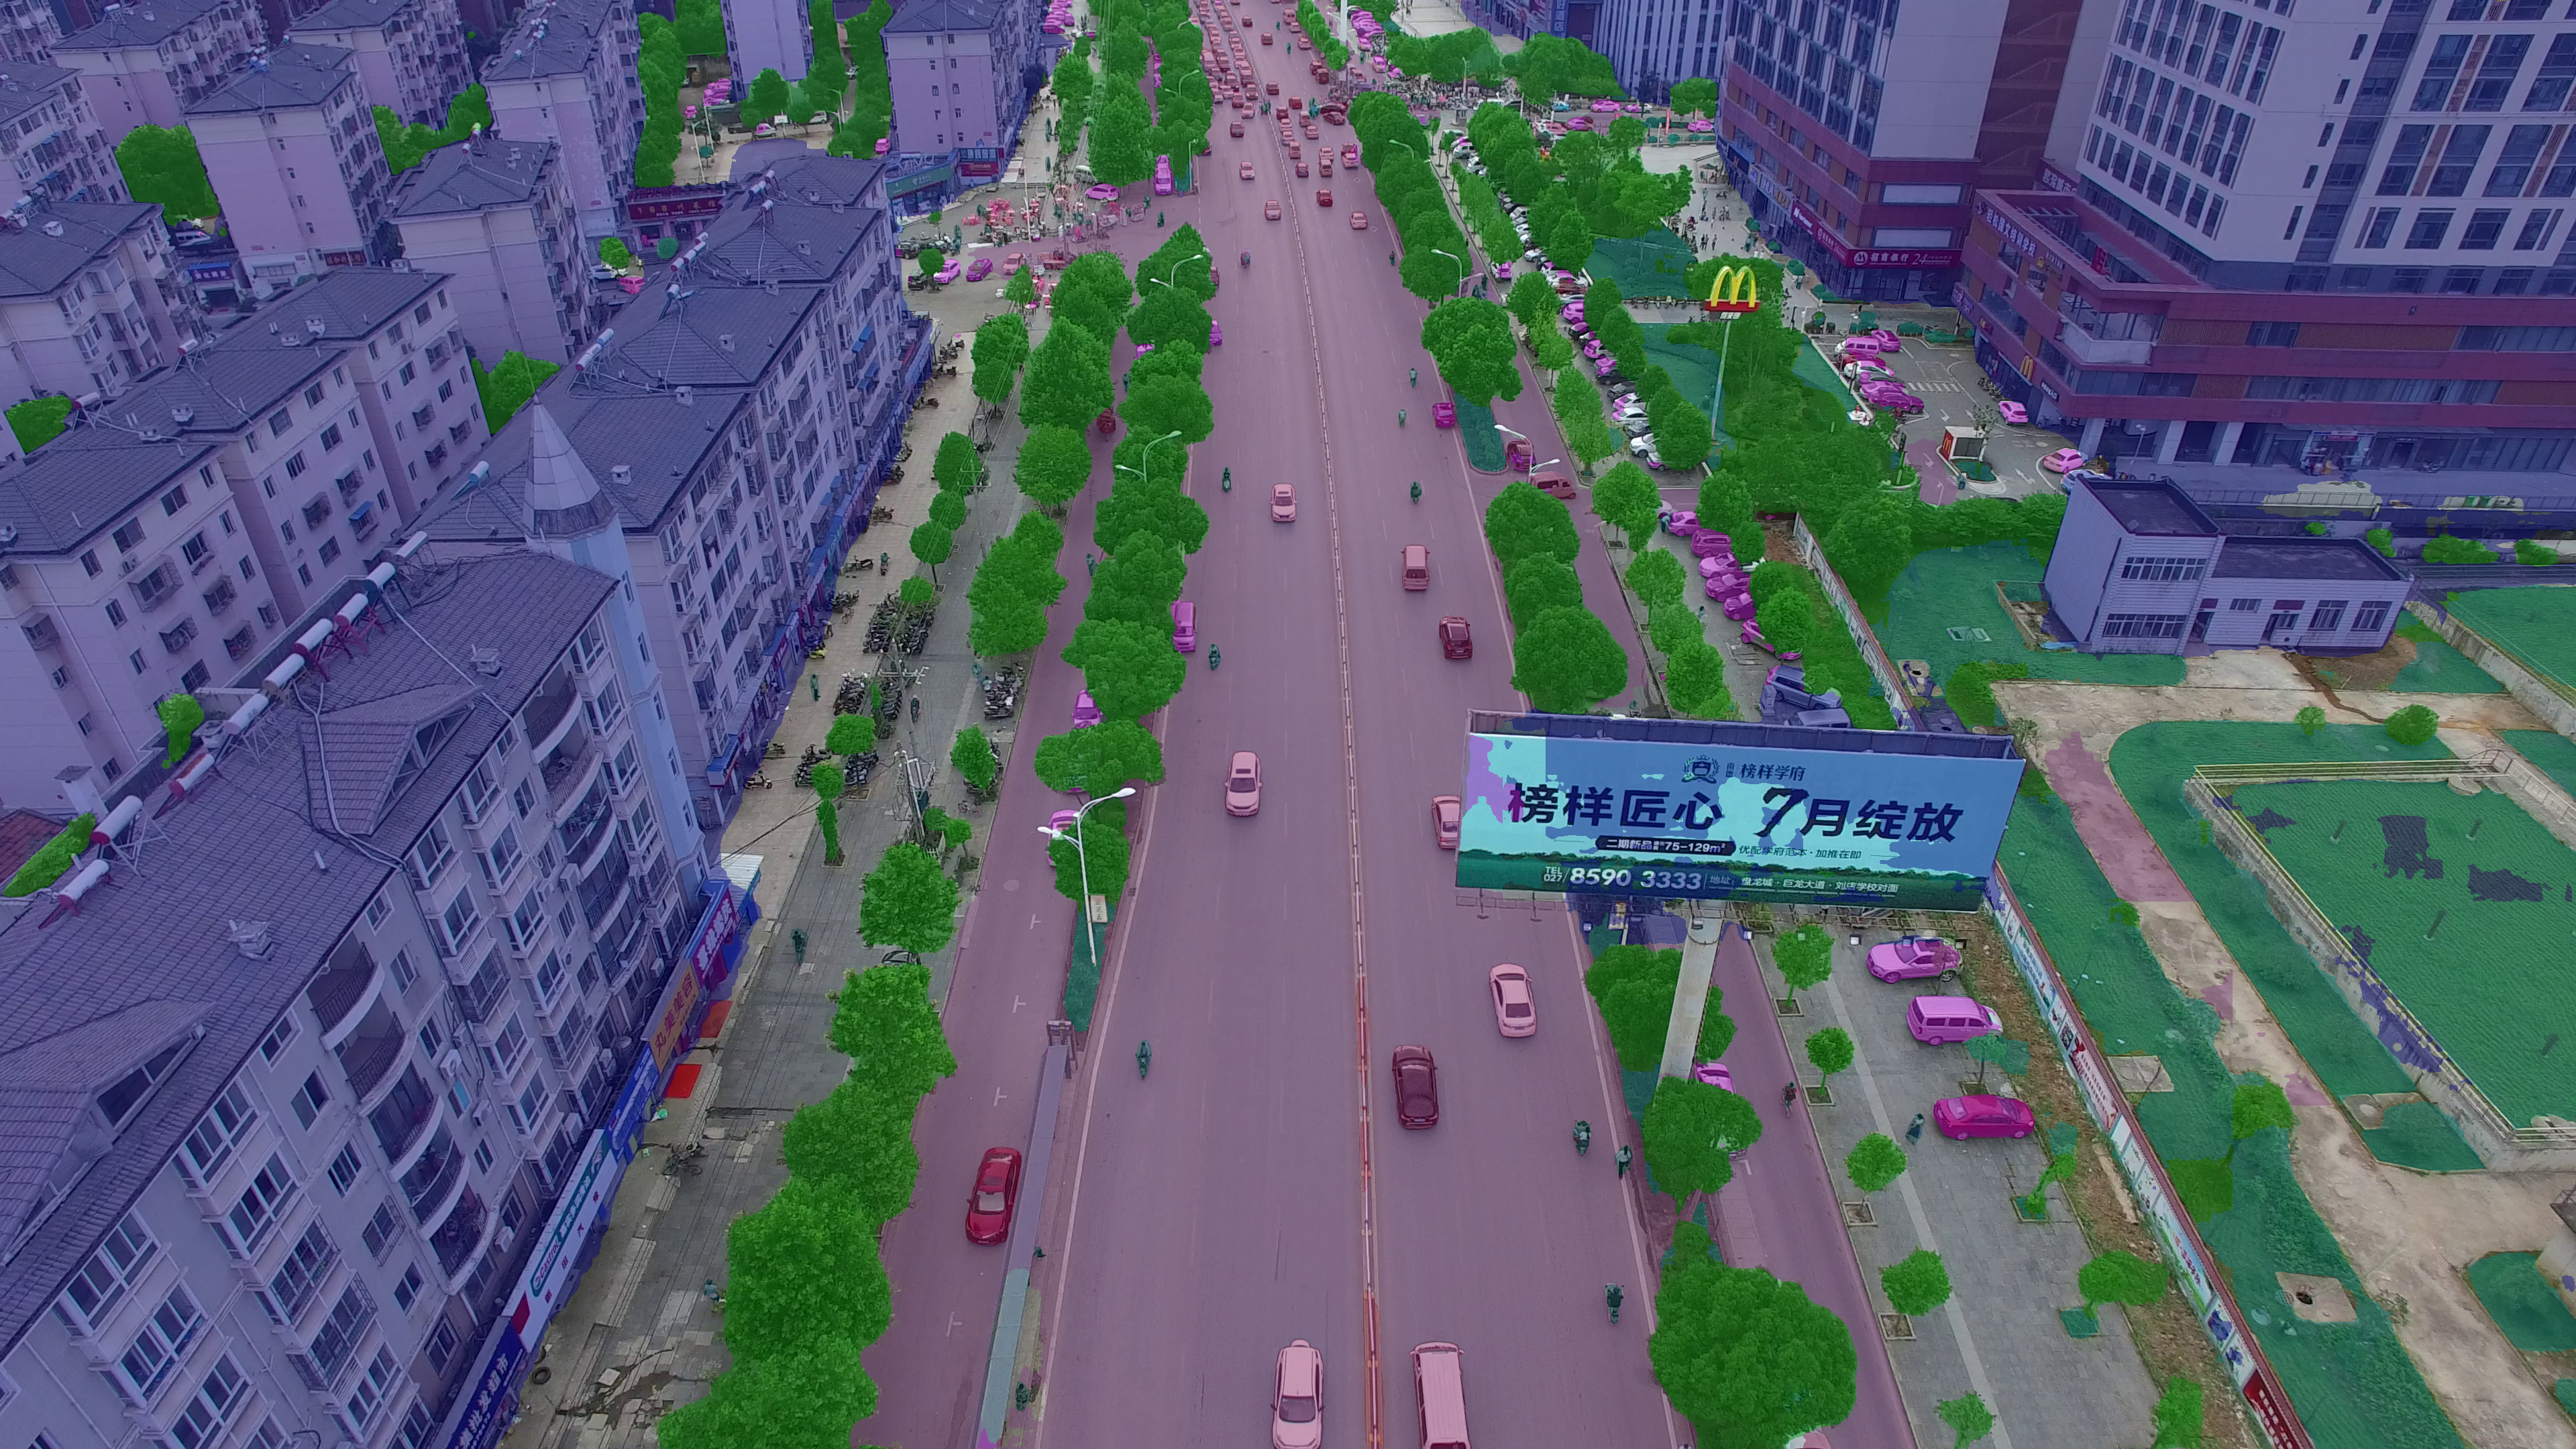
\includegraphics[width=\textwidth,height=0.35\textheight,keepaspectratio]{segmentation/000300_overlay.png}
\vspace{0.2cm}
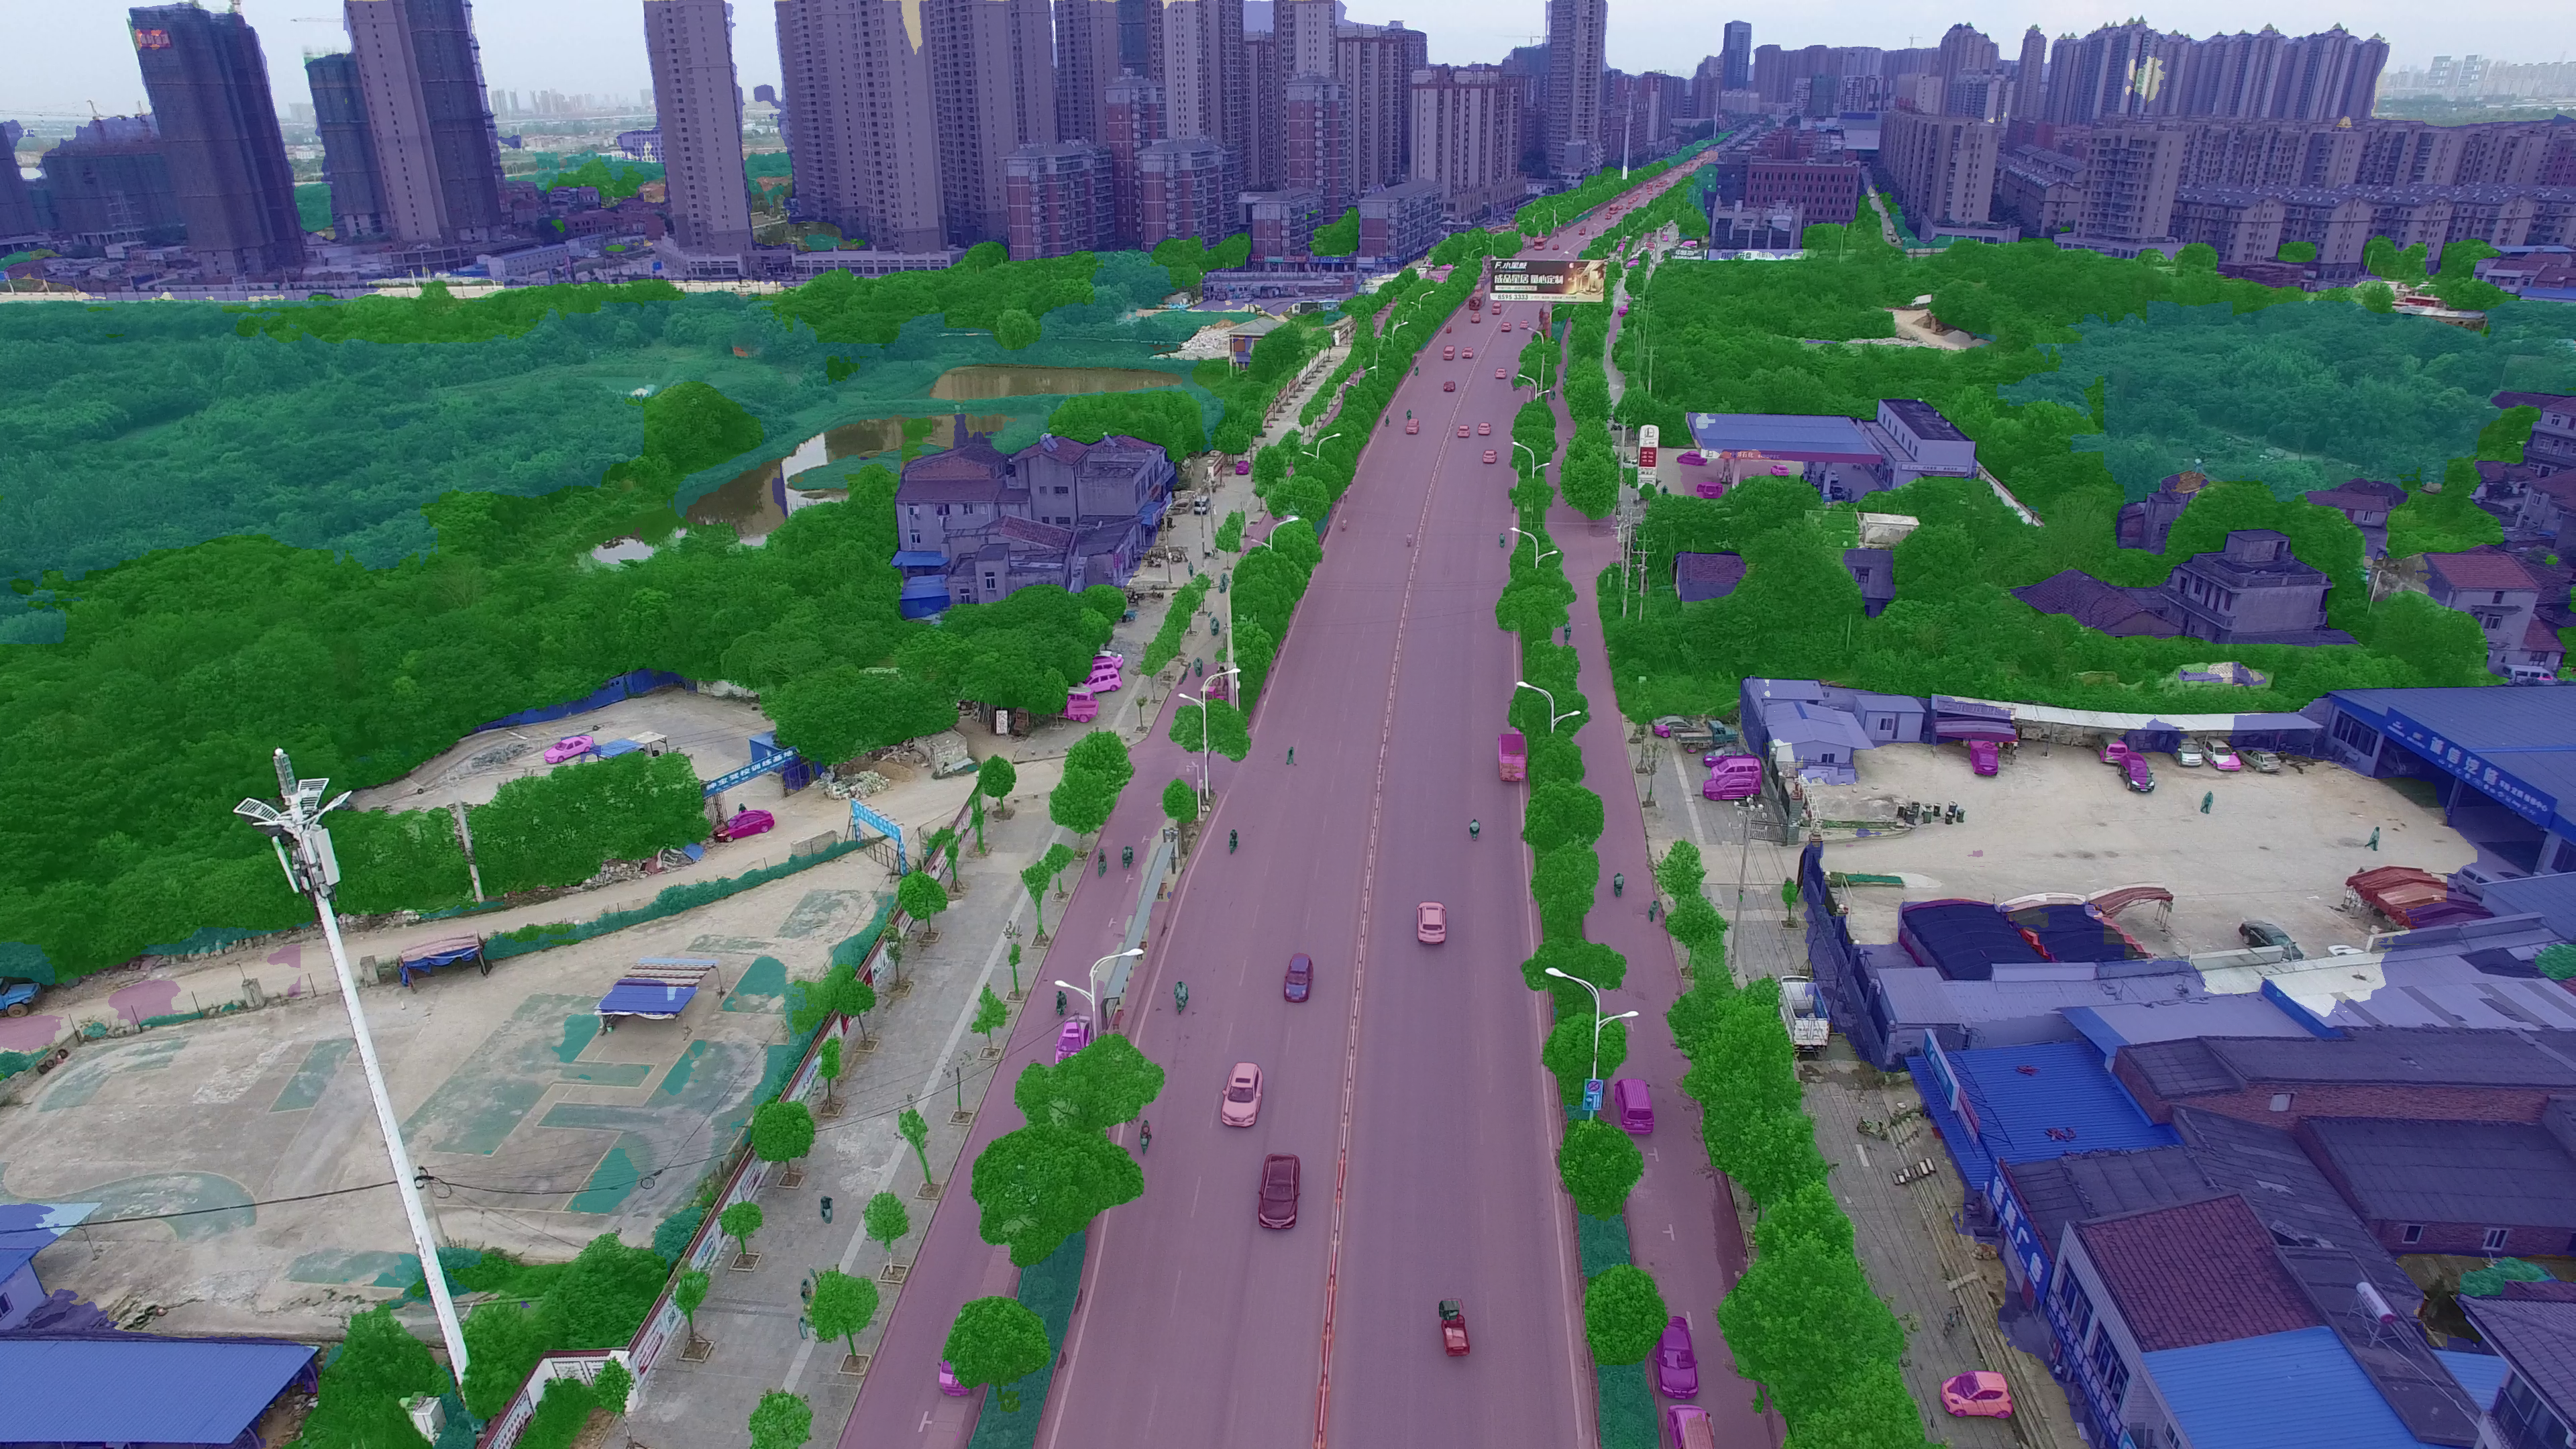
\includegraphics[width=\textwidth,height=0.35\textheight,keepaspectratio]{segmentation/000500_overlay.png}
\end{center}
\end{column}
\begin{column}{0.5\textwidth}
\begin{center}
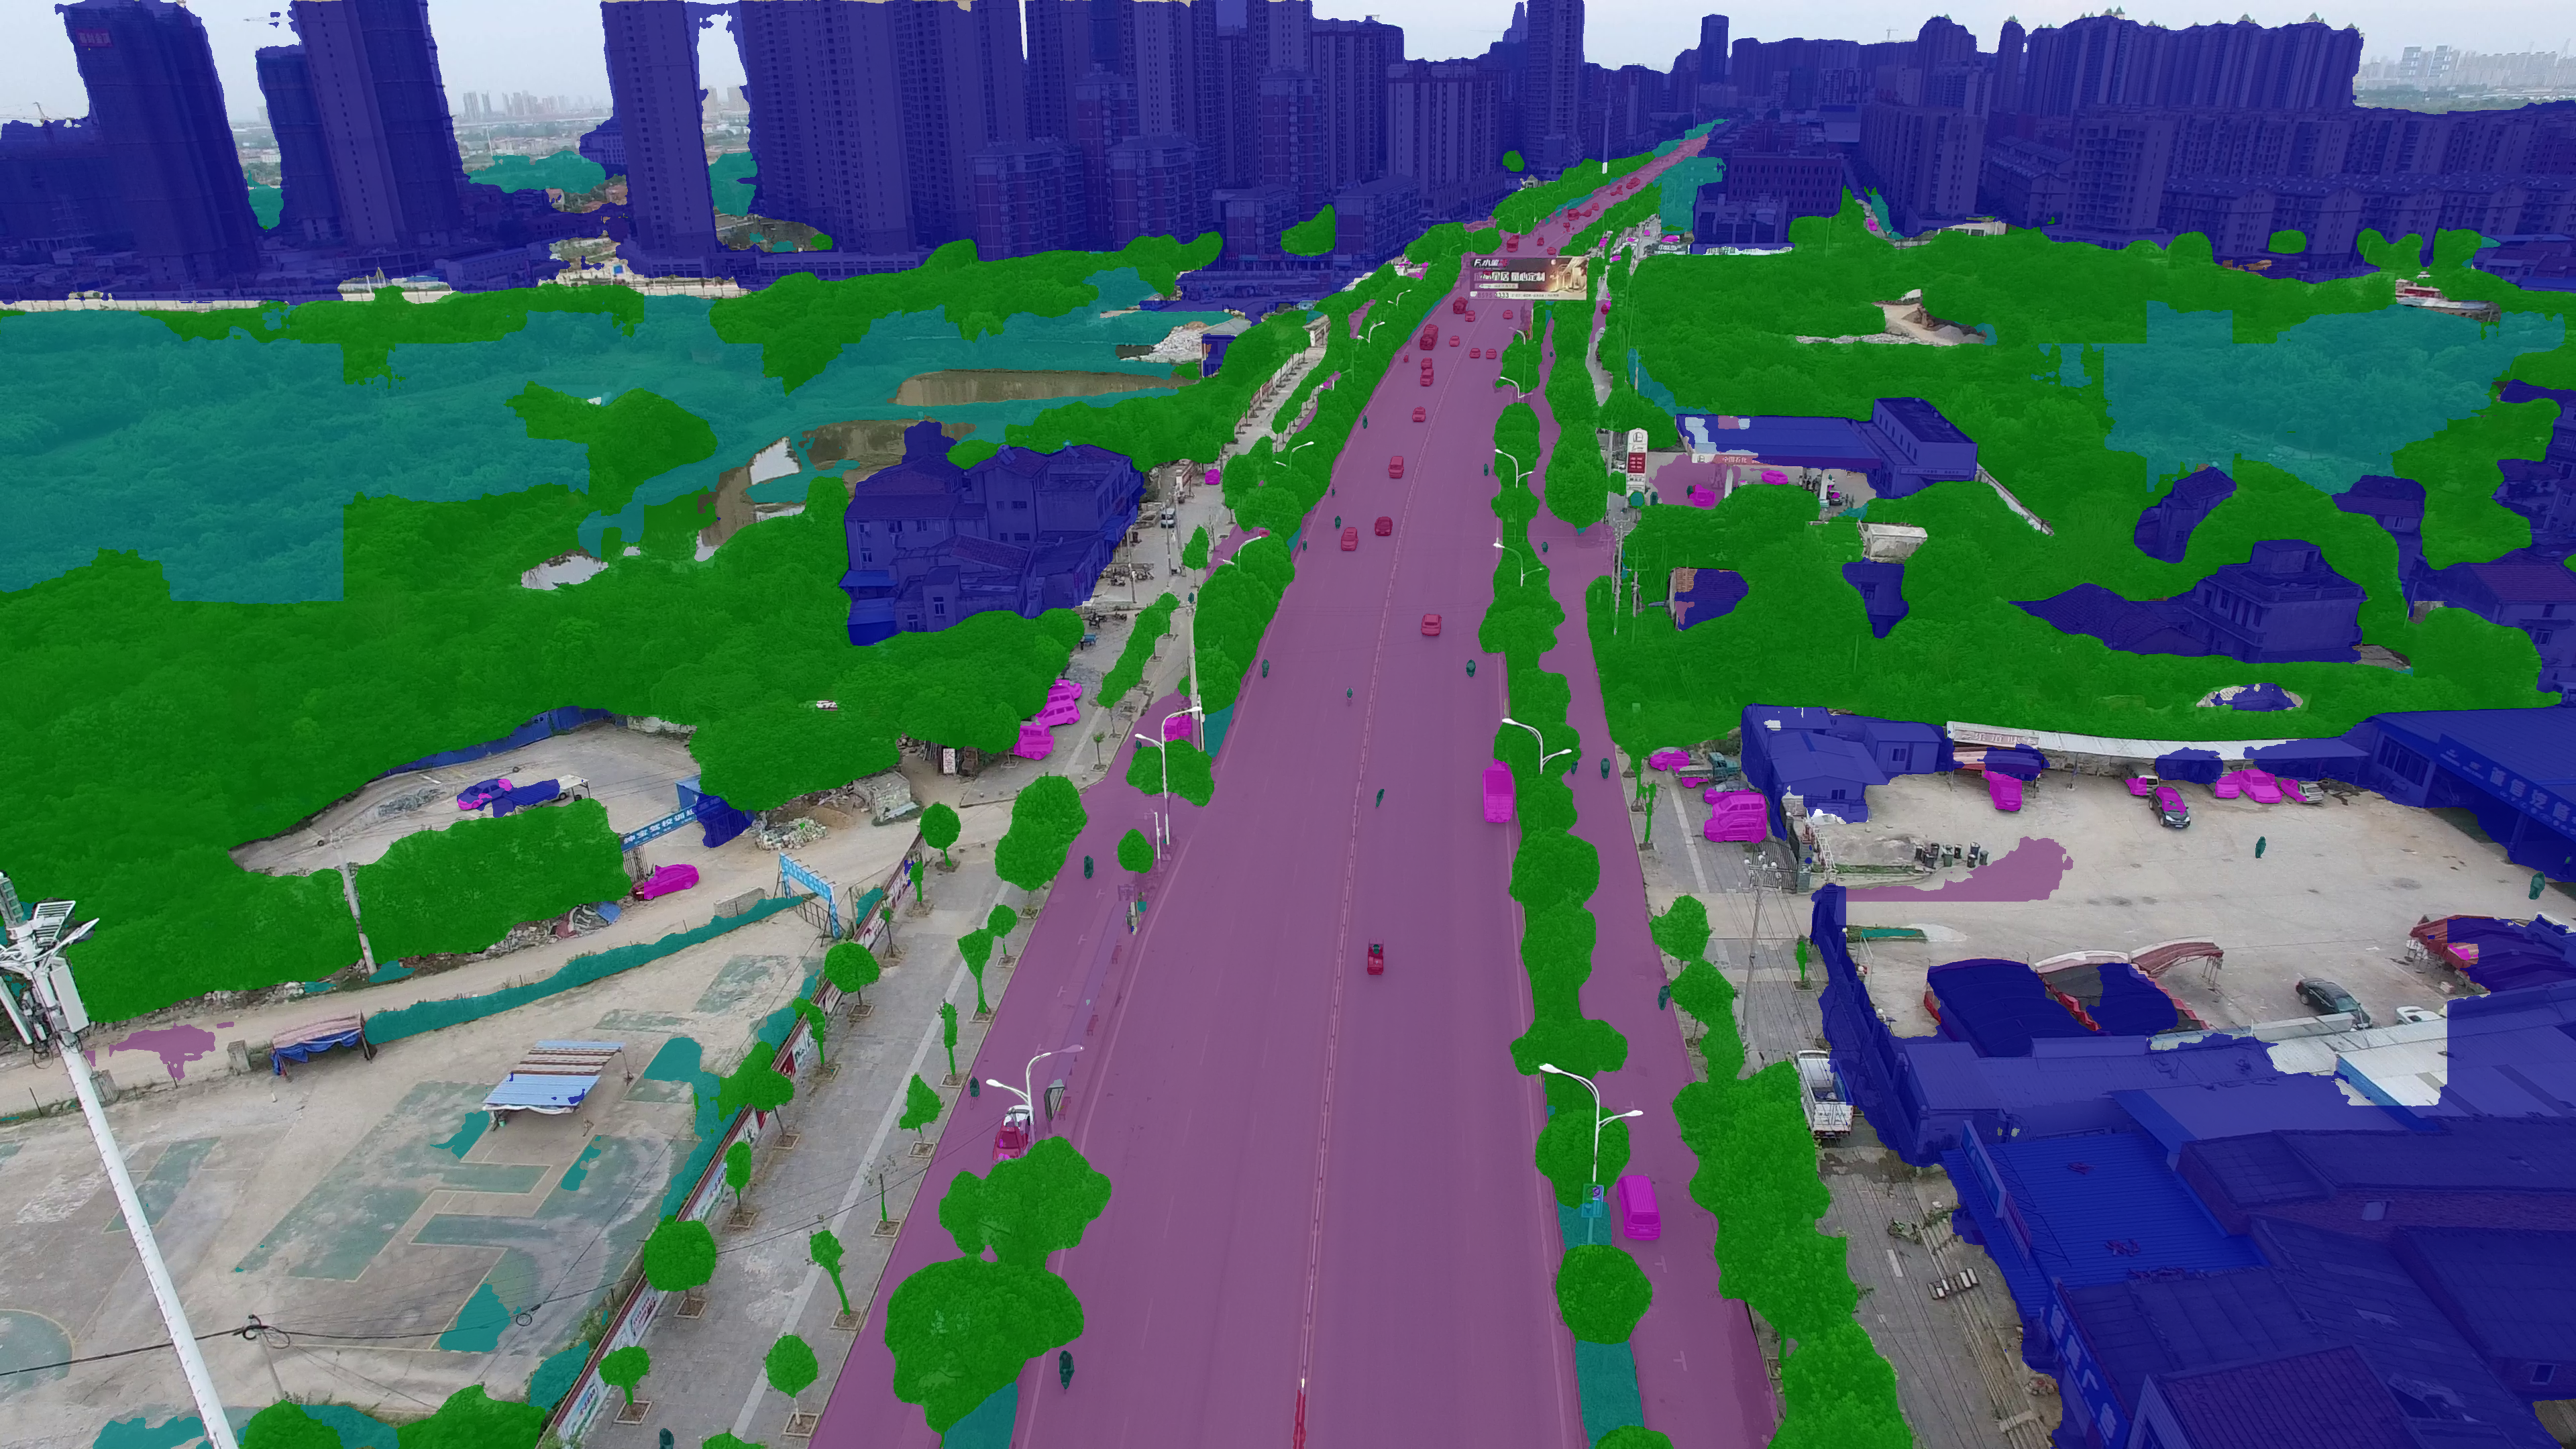
\includegraphics[width=\textwidth,height=0.35\textheight,keepaspectratio]{segmentation/000600_overlay.png}
\vspace{0.2cm}
\includegraphics[width=\textwidth,height=0.35\textheight,keepaspectratio]{segmentation/M-33-7-A-d-3-2_visualization.png}
\end{center}
\end{column}
\end{columns}
\vspace{0.3cm}
\begin{center}
\small\textit{Każdy kolor reprezentuje inną klasę obiektów}
\end{center}
\end{frame}

% -----------------------------------------------------------------------------
% Slajd: Porównanie zadań wizyjnych
% -----------------------------------------------------------------------------
\begin{frame}{Porównanie zadań -- przykład}
\textbf{Obraz: pies i dwa koty na kanapie}

\vspace{0.3cm}
\begin{tabular}{p{3.5cm}p{10cm}}
\toprule
\textbf{Zadanie} & \textbf{Wynik} \\
\midrule
Klasyfikacja & ``zwierzęta domowe'' (cały obraz, jedna etykieta) \\
\midrule
Detekcja & [bbox\_kot1, bbox\_kot2, bbox\_pies] -- 3 prostokąty \\
\midrule
Segm. semantyczna & piksele\_kot, piksele\_pies (bez rozróżnienia który kot) \\
\midrule
Segm. instancji & piksele\_kot1, piksele\_kot2, piksele\_pies (każda instancja osobno) \\
\bottomrule
\end{tabular}

\vspace{0.5cm}
\begin{center}
\small\textit{Złożoność zadania rośnie: klasyfikacja < detekcja < segmentacja semantyczna < segmentacja instancji}
\end{center}
\end{frame}

% -----------------------------------------------------------------------------
% Slajd: Porównanie zadań -- obrazek
% -----------------------------------------------------------------------------
\begin{frame}{Porównanie zadań -- wizualizacja}
\begin{center}
\includegraphics[width=0.85\textwidth,height=0.8\textheight,keepaspectratio]{classification_detection_segmentation.png}
\end{center}
\end{frame}



% -----------------------------------------------------------------------------
% Slajd: Historia - podejście dwuetapowe
% -----------------------------------------------------------------------------
\begin{frame}{Historia detekcji: podejście dwuetapowe (Two-Stage)}
\begin{center}
\includegraphics[width=0.7\textwidth,height=0.3\textheight,keepaspectratio]{one_and_two_stage_detectors.png}
\end{center}

\vspace{0.2cm}
\textbf{Era przed deep learning:} HOG + SVM, Viola-Jones (2001)

\vspace{0.2cm}
\begin{columns}
\begin{column}{0.33\textwidth}
\textbf{R-CNN (2014)}
\begin{itemize}
    \item $\sim$2000 regionów
    \item \textcolor{red}{$\sim$47s/obraz}
\end{itemize}
\end{column}
\begin{column}{0.33\textwidth}
\textbf{Fast R-CNN (2015)}
\begin{itemize}
    \item RoI Pooling
    \item \textcolor{orange}{$\sim$2s/obraz}
\end{itemize}
\end{column}
\begin{column}{0.33\textwidth}
\textbf{Faster R-CNN (2015)}
\begin{itemize}
    \item RPN network
    \item \textcolor{darkgreen}{$\sim$0.2s/obraz}
\end{itemize}
\end{column}
\end{columns}
\end{frame}

% -----------------------------------------------------------------------------
% Slajd: YOLO - rewolucja
% -----------------------------------------------------------------------------
\begin{frame}{YOLO -- rewolucja w detekcji (2016)}
\begin{center}
\Huge\textbf{``You Only Look Once''}
\end{center}

\vspace{0.5cm}
\textbf{Kluczowa innowacja:}
\begin{itemize}
    \item Detekcja jako \textbf{problem regresji}, nie klasyfikacji regionów
    \item \textbf{Jedno przejście} przez sieć neuronową
    \item Obraz dzielony na siatkę (grid) $S \times S$
    \item Każda komórka przewiduje $B$ bounding boxów + klasy
\end{itemize}

\vspace{0.5cm}
\begin{columns}
\begin{column}{0.5\textwidth}
\textbf{Two-Stage (Faster R-CNN):}
\begin{enumerate}
    \item Generuj propozycje regionów
    \item Klasyfikuj każdy region
\end{enumerate}
$\rightarrow$ Dokładne, ale wolne
\end{column}
\begin{column}{0.5\textwidth}
\textbf{One-Stage (YOLO):}
\begin{enumerate}
    \item Przewiduj wszystko naraz
\end{enumerate}
$\rightarrow$ Szybkie, real-time!
\end{column}
\end{columns}
\end{frame}

% -----------------------------------------------------------------------------
% Slajd: Jak działa YOLO - koncepcja
% -----------------------------------------------------------------------------
\begin{frame}{Jak działa YOLO -- koncepcja}
\begin{columns}
\begin{column}{0.55\textwidth}
\textbf{1. Podział obrazu na siatkę}
\begin{itemize}
    \item Obraz dzielony na $S \times S$ komórek (np. $7\times7$)
    \item Komórka ``odpowiada'' za obiekt, jeśli środek obiektu w niej leży
\end{itemize}

\vspace{0.3cm}
\textbf{2. Predykcja dla każdej komórki}
\begin{itemize}
    \item $B$ bounding boxów (x, y, w, h, confidence)
    \item $C$ prawdopodobieństw klas
    \item Wyjście: tensor $S \times S \times (B \cdot 5 + C)$
\end{itemize}

\vspace{0.3cm}
\textbf{3. Non-Maximum Suppression (NMS)}
\begin{itemize}
    \item Usuwanie duplikatów
    \item Zostawianie najlepszych detekcji
\end{itemize}
\end{column}
\begin{column}{0.45\textwidth}
\begin{center}
\begin{tikzpicture}[scale=0.8]
% Grid
\draw[step=0.7cm,gray,thin] (0,0) grid (4.9,4.9);
% Object center
\fill[red] (2.45,3.15) circle (3pt);
% Bounding box
\draw[thick,green!60!black] (1.4,1.4) rectangle (3.5,4.2);
% Label
\node[below] at (2.45,0) {\small Siatka $7\times7$};
\node[right,red] at (2.6,3.15) {\small środek};
\end{tikzpicture}
\end{center}
\end{column}
\end{columns}
\end{frame}

\begin{frame}{Architektura YOLO -- jak działa}
\begin{center}
\includegraphics[width=0.9\textwidth,height=0.45\textheight,keepaspectratio]{yolo_work2.png}
\end{center}
\end{frame}

% -----------------------------------------------------------------------------
% Slajd: Ewolucja YOLO v1-v3
% -----------------------------------------------------------------------------
\begin{frame}{Ewolucja YOLO: v1 -- v3}
\begin{tabular}{p{2cm}p{2cm}p{9cm}}
\toprule
\textbf{Wersja} & \textbf{Rok} & \textbf{Kluczowe zmiany} \\
\midrule
\textbf{YOLOv1} & 2016 & Pierwsza wersja, siatka $7\times7$, 45 FPS, problemy z małymi obiektami \\
\midrule
\textbf{YOLOv2} (YOLO9000) & 2016 & Batch normalization, anchor boxes, detekcja na wielu skalach, \href{https://www.geeksforgeeks.org/machine-learning/yolo9000-architecture-faster-stronger/}{9000 klas} \\
\midrule
\textbf{YOLOv3} & 2018 & Multi-scale predictions (3 skale), Darknet-53 backbone, lepsze małe obiekty \\
\bottomrule
\end{tabular}

\vspace{0.5cm}
\textbf{Autorzy oryginalnego YOLO:} Joseph Redmon, Ali Farhadi (University of Washington)

\vspace{0.3cm}
\textit{W 2020 roku Joseph Redmon wycofał się z prac nad CV ze względów etycznych (obawy o wykorzystanie w inwigilacji i wojsku).}
\end{frame}

% -----------------------------------------------------------------------------
% Slajd: Ewolucja YOLO v4-v5
% -----------------------------------------------------------------------------
\begin{frame}{Ewolucja YOLO: v4 -- v5}
\begin{tabular}{p{2cm}p{2cm}p{9cm}}
\toprule
\textbf{Wersja} & \textbf{Rok} & \textbf{Kluczowe zmiany} \\
\midrule
\textbf{YOLOv4} & 2020 & CSPDarknet53, PANet, Mosaic augmentation, ``Bag of Freebies'' i ``Bag of Specials'' (Alexey Bochkovskiy) \\
\midrule
\textbf{YOLOv5} & 2020 & PyTorch (nie Darknet!), auto-learning anchors, focus layer, Ultralytics \\
\midrule
\textbf{YOLOX} & 2021 & Anchor-free, decoupled head, SimOTA label assignment (Megvii) \\
\bottomrule
\end{tabular}

\vspace{0.5cm}
\textbf{Ważna zmiana:} YOLOv5 przeszło na PyTorch, co ułatwiło integrację i rozwój
\begin{itemize}
    \item Prostsze API
    \item Łatwiejszy transfer learning
    \item Aktywna społeczność i wsparcie Ultralytics
\end{itemize}
\end{frame}

% -----------------------------------------------------------------------------
% Slajd: Ewolucja YOLO v6-v8
% -----------------------------------------------------------------------------
\begin{frame}{Ewolucja YOLO: v6 -- v8}
\begin{tabular}{p{2cm}p{2cm}p{9cm}}
\toprule
\textbf{Wersja} & \textbf{Rok} & \textbf{Kluczowe zmiany} \\
\midrule
\textbf{YOLOv6} & 2022 & Meituan, EfficientRep backbone, optymalizacja dla deployment \\
\midrule
\textbf{YOLOv7} & 2022 & E-ELAN, compound scaling, auxiliary heads (autorzy YOLOv4), focal loss \\
\midrule
\textbf{YOLOv8} & 2023 & Ultralytics, anchor-free, zunifikowane API dla detection/segmentation/pose/classify/OBB \\
\bottomrule
\end{tabular}

\vspace{0.5cm}
\textbf{YOLOv8 -- przełom w użyteczności:}
\begin{itemize}
    \item Jedno API do wielu zadań
    \item Warianty: n (nano), s (small), m (medium), l (large), x (extra-large)
    \item Łatwy eksport: ONNX, TensorRT, CoreML, TFLite
\end{itemize}
\end{frame}

% -----------------------------------------------------------------------------
% Slajd: Ewolucja YOLO v9-v11
% -----------------------------------------------------------------------------
\begin{frame}{Ewolucja YOLO: v9 -- v11 (YOLO11)}
\begin{tabular}{p{2cm}p{2cm}p{9cm}}
\toprule
\textbf{Wersja} & \textbf{Rok} & \textbf{Kluczowe zmiany} \\
\midrule
\textbf{YOLOv9} & 2024 & PGI (Programmable Gradient Information), GELAN architecture \\
\midrule
\textbf{YOLOv10} & 2024 & NMS-free (eliminacja NMS), Tsinghua University \\
\midrule
\textbf{YOLO11} & 2024 & Ultralytics, C3k2 blocks, SPPF, lepszy balance accuracy/speed \\
\bottomrule
\end{tabular}

\vspace{0.5cm}
\textbf{Najnowsze trendy:}
\begin{itemize}
    \item Eliminacja NMS (Non-Maximum Suppression) dla szybszej inferencji
    \item Lepsze skalowanie modeli (n-s-m-l-x)
    \item Optymalizacja dla edge devices
\end{itemize}
\end{frame}

% -----------------------------------------------------------------------------
% Slajd: Porównanie wydajności
% -----------------------------------------------------------------------------
\begin{frame}{Porównanie wydajności -- YOLO11}
\begin{center}
\begin{tabular}{lccccc}
\toprule
\textbf{Model} & \textbf{mAP$^{val}_{50-95}$} & \textbf{CPU (ms)} & \textbf{T4 GPU (ms)} & \textbf{Params (M)} & \textbf{FLOPs (B)} \\
\midrule
YOLO11n & 39.5 & 56.1 & 1.5 & 2.6 & 6.5 \\
YOLO11s & 47.0 & 90.0 & 2.5 & 9.4 & 21.5 \\
YOLO11m & 51.5 & 183.2 & 4.7 & 20.1 & 68.0 \\
YOLO11l & 53.4 & 238.6 & 6.2 & 25.3 & 86.9 \\
YOLO11x & 54.7 & 462.8 & 11.3 & 56.9 & 194.9 \\
\bottomrule
\end{tabular}
\end{center}

\vspace{0.3cm}
\textbf{Jak czytać tabelę:}
\begin{itemize}
    \item \textbf{mAP} -- mean Average Precision na COCO dataset
    \item \textbf{n/s/m/l/x} -- rozmiary od nano do extra-large
    \item Trade-off: większy model = lepsza dokładność, ale wolniejszy
\end{itemize}
\end{frame}

% -----------------------------------------------------------------------------
% Slajd: Którą wersję wybrać?
% -----------------------------------------------------------------------------
\begin{frame}{Którą wersję YOLO wybrać?}
\textbf{Rekomendacja: YOLOv8 lub YOLO11 od Ultralytics}

\vspace{0.3cm}
\begin{tabular}{p{4cm}p{9cm}}
\toprule
\textbf{Kryterium} & \textbf{Zalecenie} \\
\midrule
Prostota użycia & YOLOv8/YOLO11 -- najlepsze API i dokumentacja \\
\midrule
Edge devices / Mobile & YOLO11n lub YOLOv8n (nano) \\
\midrule
Najlepsza dokładność & YOLO11x lub YOLOv8x \\
\midrule
Real-time na GPU & YOLO11s/m lub YOLOv8s/m \\
\midrule
Bez NMS (najszybsze) & YOLOv10 \\
\midrule
Badania naukowe & YOLOv9 (najnowsze techniki) \\
\bottomrule
\end{tabular}

\vspace{0.5cm}
\textbf{Dlaczego Ultralytics?}
\begin{itemize}
    \item Aktywny rozwój i wsparcie społeczności
    \item Zunifikowane API dla wielu zadań
    \item Doskonała dokumentacja i tutoriale
\end{itemize}
\end{frame}

% -----------------------------------------------------------------------------
% Slajd: Zadania wspierane przez YOLO
% -----------------------------------------------------------------------------
\begin{frame}{Zadania wspierane przez YOLOv8/YOLO11}
\begin{columns}
\begin{column}{0.5\textwidth}
\textbf{Detection} -- detekcja obiektów
\begin{itemize}
    \item Bounding boxes
    \item 80 klas COCO lub własne
\end{itemize}

\vspace{0.3cm}
\textbf{Segmentation} -- segmentacja instancji
\begin{itemize}
    \item Maski dla każdego obiektu
    \item Pixel-perfect granice
\end{itemize}

\vspace{0.3cm}
\textbf{Classification} -- klasyfikacja obrazów
\begin{itemize}
    \item Cały obraz → jedna klasa
\end{itemize}
\end{column}
\begin{column}{0.5\textwidth}
\textbf{Pose Estimation} -- estymacja pozy
\begin{itemize}
    \item 17 keypoints (COCO format)
    \item Śledzenie ruchu człowieka
\end{itemize}

\vspace{0.3cm}
\textbf{OBB} -- Oriented Bounding Boxes
\begin{itemize}
    \item Obrócone prostokąty
    \item Dla obiektów pod kątem
\end{itemize}

\vspace{0.3cm}
\textbf{Tracking} -- śledzenie obiektów
\begin{itemize}
    \item ByteTrack, BoT-SORT
    \item Tożsamość obiektów w czasie
\end{itemize}
\end{column}
\end{columns}
\end{frame}

% -----------------------------------------------------------------------------
% Slajd: Podsumowanie części 1
% -----------------------------------------------------------------------------
\begin{frame}{Podsumowanie: Wprowadzenie i kontekst}
\begin{itemize}
    \item \textbf{Klasyfikacja} -- jedna etykieta na obraz
    \item \textbf{Detekcja} -- lokalizacja wielu obiektów (bounding boxes)
    \item \textbf{Segmentacja} -- klasyfikacja na poziomie pikseli
\end{itemize}

\vspace{0.3cm}
\begin{itemize}
    \item \textbf{Two-stage} (R-CNN family) -- dokładne, ale wolne
    \item \textbf{One-stage} (YOLO) -- szybkie, real-time
\end{itemize}

\vspace{0.3cm}
\begin{itemize}
    \item YOLO przeszło ogromną ewolucję: v1 (2016) → YOLO11 (2024)
    \item \textbf{Ultralytics YOLOv8/YOLO11} -- najlepszy wybór do praktycznych zastosowań
    \item Warianty n-s-m-l-x pozwalają dopasować model do wymagań
\end{itemize}

\vspace{0.5cm}
\begin{center}
\textbf{W następnej części: Architektura YOLO i jak działa od środka}
\end{center}
\end{frame}

% =============================================================================
% CZĘŚĆ 2: ARCHITEKTURA SIECI
% =============================================================================
\section{Architektura sieci}

% -----------------------------------------------------------------------------
% Slajd: Wprowadzenie do sieci neuronowych
% -----------------------------------------------------------------------------
\begin{frame}{Krótkie przypomnienie: sieci neuronowe}
\begin{columns}
\begin{column}{0.45\textwidth}
% OBRAZEK: neural_network_diagram.png
% Szukaj: "neural network layers diagram simple"
% Opis: Prosty schemat sieci neuronowej (input-hidden-output)
% Ścieżka: img/neural_network_diagram.png
\begin{center}
\includegraphics[width=0.9\textwidth,height=0.45\textheight,keepaspectratio]{img/neural_network_diagram.png}
\end{center}
\vspace{0.2cm}
\textbf{Interaktywna wizualizacja:}\\\url{https://playground.tensorflow.org/}
\end{column}
\begin{column}{0.55\textwidth}
\textbf{Podstawowe pojęcia:}
\begin{itemize}
    \item \textbf{Neurony} -- jednostki obliczeniowe
    \item \textbf{Wagi (weights)} -- parametry do nauki
    \item \textbf{Bias} -- przesunięcie aktywacji
    \item \textbf{Funkcja aktywacji} -- nieliniowość (ReLU, Sigmoid, Mish)
\end{itemize}

\vspace{0.3cm}
\textbf{Warstwy konwolucyjne (Conv):}
\begin{itemize}
    \item Filtry wykrywające wzorce
    \item Zachowują informację przestrzenną
    \item Współdzielenie wag $\rightarrow$ efektywność
\end{itemize}
\end{column}
\end{columns}
\end{frame}

% -----------------------------------------------------------------------------
% Slajd: Sieci neuronowe - operacje
% -----------------------------------------------------------------------------
\begin{frame}{Sieci neuronowe -- kluczowe operacje}
\begin{columns}
\begin{column}{0.5\textwidth}
% OBRAZEK: convolution_visualization.png
% Szukaj: "convolution operation visualization CNN"
% Opis: Wizualizacja operacji konwolucji z filtrem przesuwającym się po obrazie
% Ścieżka: img/convolution_visualization.png
\begin{center}
\includegraphics[width=0.9\textwidth,height=0.45\textheight,keepaspectratio]{img/convolution_visualization.png}
\end{center}
\end{column}
\begin{column}{0.5\textwidth}
\textbf{Kluczowe operacje w CNN:}
\begin{itemize}
    \item \textbf{Convolution} -- ekstrakcja cech
    \item \textbf{Pooling} -- redukcja rozmiaru
    \item \textbf{Batch Normalization} -- stabilizacja treningu
    \item \textbf{Skip connections} -- przepływ gradientów
\end{itemize}

\vspace{0.3cm}
\textbf{Parametry sieci:}
\begin{itemize}
    \item Liczba warstw (depth)
    \item Liczba filtrów (width)
    \item Rozmiar filtra (kernel size - nieparzyste)
\end{itemize}
\end{column}
\end{columns}
\end{frame}

\begin{frame}{Kluczowe operacje}
    \begin{center}
\includegraphics[width=0.9\textwidth,height=0.7\textheight,keepaspectratio]{img/schemat_ogolny.png}
\end{center}
\end{frame}

\begin{frame}{Pooling}
    \begin{center}
\includegraphics[width=0.9\textwidth,height=0.7\textheight,keepaspectratio]{img/pooling.png}
\end{center}
\end{frame}



% -----------------------------------------------------------------------------
% Slajd: Architektura YOLO - przegląd
% -----------------------------------------------------------------------------
\begin{frame}{Architektura YOLO -- przegląd}
\begin{center}
\includegraphics[width=0.9\textwidth,height=0.45\textheight,keepaspectratio]{yolo_architecture.png}
\end{center}

\vspace{0.3cm}
\textbf{Trzy główne komponenty:}
\begin{enumerate}
    \item \textbf{Backbone} -- ekstraktor cech (``kręgosłup'' sieci)
    \item \textbf{Neck} -- agregacja cech z różnych skal
    \item \textbf{Head} -- warstwa detekcyjna (predykcja bbox + klasy)
\end{enumerate}
\end{frame}



% -----------------------------------------------------------------------------
% Slajd: Backbone
% -----------------------------------------------------------------------------
\begin{frame}{Backbone -- ekstraktor cech}
\textbf{Zadanie:} Przetworzenie obrazu na hierarchię map cech (feature maps)

\vspace{0.3cm}
\begin{columns}
\begin{column}{0.5\textwidth}
\textbf{Popularne backbone'y w YOLO:}
\begin{itemize}
    \item \textbf{Darknet-53} (YOLOv3) -- 53 warstwy, residual blocks
    \item \textbf{CSPDarknet} (YOLOv4/v5) -- Cross-Stage Partial connections
    \item \textbf{EfficientRep} (YOLOv6) -- reparametryzacja dla szybkości
    \item \textbf{E-ELAN} (YOLOv7) -- Extended ELAN
    \item \textbf{C2f} (YOLOv8) -- ulepszone CSP
\end{itemize}
\end{column}
\begin{column}{0.5\textwidth}
\textbf{Co daje backbone:}
\begin{itemize}
    \item Wczesne warstwy: krawędzie, tekstury
    \item Środkowe warstwy: części obiektów
    \item Późne warstwy: semantyka wysokiego poziomu
\end{itemize}

\vspace{0.3cm}
\textbf{Feature maps:}\\
Rozdzielczość maleje, liczba kanałów rośnie
\begin{center}
$640 \times 640 \times 3 \rightarrow 20 \times 20 \times 1024$
\end{center}
\end{column}
\end{columns}
\end{frame}

% -----------------------------------------------------------------------------
% Slajd: CSP (Cross-Stage Partial)
% -----------------------------------------------------------------------------
\begin{frame}{CSP -- Cross-Stage Partial Networks}
\textbf{Problem:} Duże sieci $\rightarrow$ dużo obliczeń, redundancja gradientów

\vspace{0.3cm}
\textbf{Rozwiązanie CSP:}
\begin{itemize}
    \item Dzieli feature map na dwie części
    \item Jedna część przechodzi przez gęste bloki
    \item Druga część ``przeskakuje'' (shortcut)
    \item Łączenie na końcu (concatenation)
\end{itemize}

\vspace{0.3cm}
\begin{center}
\begin{tikzpicture}[scale=0.9]
\node[draw, rectangle, fill=blue!20, minimum width=1.5cm, minimum height=1cm] (input) at (0,0) {Input};
\node[draw, rectangle, fill=green!20, minimum width=1cm, minimum height=0.5cm] (part1) at (2,0.5) {Part 1};
\node[draw, rectangle, fill=green!20, minimum width=1cm, minimum height=0.5cm] (part2) at (2,-0.5) {Part 2};
\node[draw, rectangle, fill=orange!20, minimum width=1.5cm, minimum height=0.5cm] (dense) at (4,0.5) {Dense Block};
\node[draw, rectangle, fill=red!20, minimum width=1.5cm, minimum height=1cm] (concat) at (6.5,0) {Concat};

\draw[->, thick] (input) -- (1.2,0) -- (1.2,0.5) -- (part1);
\draw[->, thick] (1.2,0) -- (1.2,-0.5) -- (part2);
\draw[->, thick] (part1) -- (dense);
\draw[->, thick] (dense) -- (5.5,0.5) -- (5.5,0.3) -- (concat);
\draw[->, thick] (part2) -- (5.5,-0.5) -- (5.5,-0.3) -- (concat);
\end{tikzpicture}
\end{center}

\vspace{0.3cm}
\textbf{Korzyści:} Mniej obliczeń, lepszy przepływ gradientów, lepsza generalizacja
\end{frame}

% -----------------------------------------------------------------------------
% Slajd: Neck - FPN
% -----------------------------------------------------------------------------
\begin{frame}{Neck: Feature Pyramid Network (FPN)}
\textbf{Problem:} Obiekty różnych rozmiarów wymagają cech z różnych skal

\vspace{0.3cm}
\begin{columns}
\begin{column}{0.55\textwidth}
\textbf{Idea FPN:}
\begin{itemize}
    \item \textbf{Bottom-up pathway:} backbone (encoder)
    \item \textbf{Top-down pathway:} upsampling głębokich cech
    \item \textbf{Lateral connections:} łączenie cech z obu ścieżek
\end{itemize}

\vspace{0.3cm}
\textbf{Wynik:}
\begin{itemize}
    \item Duża rozdzielczość + głęboka semantyka
    \item Lepsza detekcja małych obiektów
    \item Multi-scale predictions
\end{itemize}
\end{column}
\begin{column}{0.45\textwidth}
\begin{center}
\begin{tikzpicture}[scale=0.7]
% Bottom-up (left)
\node[draw, fill=blue!30, minimum width=2cm, minimum height=0.5cm] (c2) at (0,0) {\tiny C2 (duża)};
\node[draw, fill=blue!40, minimum width=1.6cm, minimum height=0.5cm] (c3) at (0,-1) {\tiny C3};
\node[draw, fill=blue!50, minimum width=1.2cm, minimum height=0.5cm] (c4) at (0,-2) {\tiny C4};
\node[draw, fill=blue!60, minimum width=0.8cm, minimum height=0.5cm] (c5) at (0,-3) {\tiny C5 (mała)};

% Top-down (right)
\node[draw, fill=orange!30, minimum width=2cm, minimum height=0.5cm] (p2) at (4,0) {\tiny P2};
\node[draw, fill=orange!40, minimum width=1.6cm, minimum height=0.5cm] (p3) at (4,-1) {\tiny P3};
\node[draw, fill=orange!50, minimum width=1.2cm, minimum height=0.5cm] (p4) at (4,-2) {\tiny P4};
\node[draw, fill=orange!60, minimum width=0.8cm, minimum height=0.5cm] (p5) at (4,-3) {\tiny P5};

% Arrows
\draw[->, thick] (c2) -- (c3);
\draw[->, thick] (c3) -- (c4);
\draw[->, thick] (c4) -- (c5);

\draw[->, thick, dashed] (p5) -- (p4);
\draw[->, thick, dashed] (p4) -- (p3);
\draw[->, thick, dashed] (p3) -- (p2);

\draw[->, thick, green!60!black] (c5) -- (p5);
\draw[->, thick, green!60!black] (c4) -- (p4);
\draw[->, thick, green!60!black] (c3) -- (p3);
\draw[->, thick, green!60!black] (c2) -- (p2);

\node[below] at (0,-3.5) {\tiny Backbone};
\node[below] at (4,-3.5) {\tiny FPN};
\end{tikzpicture}
\end{center}
\end{column}
\end{columns}
\end{frame}

% -----------------------------------------------------------------------------
% Slajd: Neck - PANet
% -----------------------------------------------------------------------------
\begin{frame}{Neck: Path Aggregation Network (PANet)}
\textbf{Rozszerzenie FPN:} Dodatkowa ścieżka bottom-up

\vspace{0.3cm}
\begin{columns}
\begin{column}{0.5\textwidth}
\textbf{PANet dodaje:}
\begin{itemize}
    \item Druga ścieżka bottom-up po FPN
    \item Krótsza droga dla niskich cech
    \item Adaptive feature pooling
\end{itemize}

\vspace{0.3cm}
\textbf{Dlaczego to pomaga:}
\begin{itemize}
    \item Cechy z wczesnych warstw (krawędzie) szybciej docierają do głowy
    \item Lepsza lokalizacja precyzyjnych granic
    \item Używane w YOLOv4, v5, v8
\end{itemize}
\end{column}
\begin{column}{0.5\textwidth}
\begin{center}
\begin{tikzpicture}[scale=0.6]
% Backbone
\node[draw, fill=blue!30, minimum width=1.5cm, minimum height=0.4cm] (b1) at (0,0) {\tiny Low};
\node[draw, fill=blue!50, minimum width=1.2cm, minimum height=0.4cm] (b2) at (0,-1) {\tiny Mid};
\node[draw, fill=blue!70, minimum width=0.9cm, minimum height=0.4cm] (b3) at (0,-2) {\tiny High};

% FPN (top-down)
\node[draw, fill=orange!30, minimum width=1.5cm, minimum height=0.4cm] (f1) at (2.5,0) {\tiny P3};
\node[draw, fill=orange!50, minimum width=1.2cm, minimum height=0.4cm] (f2) at (2.5,-1) {\tiny P4};
\node[draw, fill=orange!70, minimum width=0.9cm, minimum height=0.4cm] (f3) at (2.5,-2) {\tiny P5};

% PANet (bottom-up)
\node[draw, fill=green!30, minimum width=1.5cm, minimum height=0.4cm] (p1) at (5,0) {\tiny N3};
\node[draw, fill=green!50, minimum width=1.2cm, minimum height=0.4cm] (p2) at (5,-1) {\tiny N4};
\node[draw, fill=green!70, minimum width=0.9cm, minimum height=0.4cm] (p3) at (5,-2) {\tiny N5};

% Arrows
\draw[->, thick] (b1) -- (b2);
\draw[->, thick] (b2) -- (b3);

\draw[->, thick, dashed] (f3) -- (f2);
\draw[->, thick, dashed] (f2) -- (f1);

\draw[->, thick, dotted, red] (p1) -- (p2);
\draw[->, thick, dotted, red] (p2) -- (p3);

\draw[->, thick] (b3) -- (f3);
\draw[->, thick] (b2) -- (f2);
\draw[->, thick] (b1) -- (f1);

\draw[->, thick] (f1) -- (p1);
\draw[->, thick] (f2) -- (p2);
\draw[->, thick] (f3) -- (p3);

\node[below] at (0,-2.5) {\tiny Backbone};
\node[below] at (2.5,-2.5) {\tiny FPN};
\node[below] at (5,-2.5) {\tiny PANet};
\end{tikzpicture}
\end{center}
\end{column}
\end{columns}
\end{frame}

% -----------------------------------------------------------------------------
% Slajd: Head - warstwa detekcyjna
% -----------------------------------------------------------------------------
\begin{frame}{Head -- warstwa detekcyjna}
\textbf{Zadanie:} Przekształcenie cech w finalne predykcje

\vspace{0.3cm}
\begin{columns}
\begin{column}{0.5\textwidth}
\textbf{Coupled Head (starsze YOLO):}
\begin{itemize}
    \item Wspólna ścieżka dla klasyfikacji i lokalizacji
    \item Prostsze, ale może być suboptymalne
\end{itemize}

\vspace{0.3cm}
\textbf{Decoupled Head (YOLOX, v8):}
\begin{itemize}
    \item \textbf{Osobna gałąź} dla klasyfikacji
    \item \textbf{Osobna gałąź} dla bbox regression
    \item \textbf{Osobna gałąź} dla objectness
    \item Lepsza konwergencja
\end{itemize}
\end{column}
\begin{column}{0.5\textwidth}
\textbf{Wyjście Head (per skala):}

Dla siatki $H \times W$:
\begin{itemize}
    \item \textbf{Bbox:} $H \times W \times 4$ (x, y, w, h)
    \item \textbf{Objectness:} $H \times W \times 1$
    \item \textbf{Classes:} $H \times W \times C$
\end{itemize}

\vspace{0.3cm}
\textbf{Multi-scale (3 skale):}
\begin{itemize}
    \item $80\times80$ -- małe obiekty
    \item $40\times40$ -- średnie obiekty
    \item $20\times20$ -- duże obiekty
\end{itemize}
\end{column}
\end{columns}
\end{frame}

% -----------------------------------------------------------------------------
% Slajd: Anchor boxes
% -----------------------------------------------------------------------------
\begin{frame}{Anchor Boxes -- co to jest?}
\textbf{Idea:} Predefiniowane ``szablony'' bounding boxów różnych kształtów

\vspace{0.3cm}
\begin{columns}
\begin{column}{0.55\textwidth}
\textbf{Dlaczego anchory:}
\begin{itemize}
    \item Sieć nie przewiduje absolutnych współrzędnych
    \item Przewiduje \textbf{offsety} względem anchorów
    \item Łatwiejsze do nauki (mniejsze wartości)
\end{itemize}

\vspace{0.3cm}
\textbf{Typowe anchory (YOLOv5):}
\begin{itemize}
    \item Mała skala: (10,13), (16,30), (33,23)
    \item Średnia: (30,61), (62,45), (59,119)
    \item Duża: (116,90), (156,198), (373,326)
\end{itemize}

\vspace{0.3cm}
\textbf{Auto-anchor:} YOLOv5+ automatycznie dopasowuje anchory do datasetu (k-means)
\end{column}
\begin{column}{0.45\textwidth}
\begin{center}
\begin{tikzpicture}[scale=0.8]
% Grid cell
\draw[thick, fill=gray!10] (0,0) rectangle (3,3);
\node at (1.5,3.3) {\small Komórka siatki};

% Anchors
\draw[thick, blue, dashed] (0.5,0.5) rectangle (2.5,2.8);
\draw[thick, red, dashed] (0.3,1) rectangle (2.7,2.2);
\draw[thick, green!60!black, dashed] (0.8,0.3) rectangle (2.2,2.5);

% Center
\fill[black] (1.5,1.5) circle (3pt);

\node[right, blue] at (3.1,2.5) {\tiny Anchor 1};
\node[right, red] at (3.1,1.6) {\tiny Anchor 2};
\node[right, green!60!black] at (3.1,0.7) {\tiny Anchor 3};
\end{tikzpicture}
\end{center}
\end{column}
\end{columns}
\end{frame}

% -----------------------------------------------------------------------------
% Slajd: Anchor-free
% -----------------------------------------------------------------------------
\begin{frame}{Anchor-Free -- nowoczesne podejście}
\textbf{Problem z anchorami:}
\begin{itemize}
    \item Wymagają ręcznego doboru lub k-means
    \item Dużo hiperparametrów
    \item Problemy z obiektami o nietypowych proporcjach
\end{itemize}

\vspace{0.3cm}
\textbf{Anchor-free (YOLOX, YOLOv8, YOLO11):}
\begin{itemize}
    \item Bezpośrednia predykcja środka obiektu
    \item Predykcja szerokości i wysokości bez anchorów
    \item Prostszy model, mniej hiperparametrów
\end{itemize}

\vspace{0.3cm}
\begin{columns}
\begin{column}{0.5\textwidth}
\textbf{Anchor-based:}
\[
\hat{x} = \sigma(t_x) + c_x
\]
\[
\hat{w} = a_w \cdot e^{t_w}
\]
\end{column}
\begin{column}{0.5\textwidth}
\textbf{Anchor-free:}
\[
\hat{x} = \sigma(t_x) \cdot s + c_x \cdot s
\]
\[
\hat{w} = e^{t_w} \cdot s
\]
\small gdzie $s$ = stride danej skali
\end{column}
\end{columns}
\end{frame}

% -----------------------------------------------------------------------------
% Slajd: Multi-scale predictions
% -----------------------------------------------------------------------------
\begin{frame}{Multi-Scale Predictions -- dlaczego 3 skale?}
\begin{columns}
\begin{column}{0.5\textwidth}
\textbf{Problem:}
\begin{itemize}
    \item Małe obiekty -- mało pikseli, trudne do wykrycia
    \item Duże obiekty -- mogą wykraczać poza receptive field
    \item Jedna skala nie pasuje do wszystkich
\end{itemize}

\vspace{0.3cm}
\textbf{Rozwiązanie -- 3 skale:}
\begin{itemize}
    \item \textbf{P3 ($80\times80$):} stride 8, małe obiekty
    \item \textbf{P4 ($40\times40$):} stride 16, średnie obiekty
    \item \textbf{P5 ($20\times20$):} stride 32, duże obiekty
\end{itemize}
\end{column}
\begin{column}{0.5\textwidth}
\begin{center}
\begin{tikzpicture}[scale=0.6]
% P3
\draw[thick, fill=green!20] (0,0) grid[step=0.3] (2.4,2.4);
\node[below] at (1.2,-0.2) {\tiny P3: $80\times80$};
\node[above] at (1.2,2.6) {\tiny małe obj.};

% P4
\draw[thick, fill=yellow!20] (3,0.3) grid[step=0.45] (4.8,2.1);
\node[below] at (3.9,-0.2) {\tiny P4: $40\times40$};
\node[above] at (3.9,2.6) {\tiny średnie};

% P5
\draw[thick, fill=red!20] (5.5,0.6) grid[step=0.6] (6.7,1.8);
\node[below] at (6.1,-0.2) {\tiny P5: $20\times20$};
\node[above] at (6.1,2.6) {\tiny duże obj.};
\end{tikzpicture}
\end{center}

\vspace{0.3cm}
\textbf{Przypisanie obiektów:}\\
Obiekt przypisany do skali, gdzie jego rozmiar najlepiej pasuje do receptive field
\end{column}
\end{columns}
\end{frame}

% =============================================================================
% CZĘŚĆ 3: JAK DZIAŁA PREDYKCJA
% =============================================================================
\section{Jak działa predykcja}

% -----------------------------------------------------------------------------
% Slajd: Pipeline predykcji
% -----------------------------------------------------------------------------
\begin{frame}{Pipeline predykcji YOLO}
\begin{center}
\begin{tikzpicture}[scale=0.9, every node/.style={font=\small}]
% Boxes
\node[draw, rectangle, fill=blue!20, minimum width=2cm, minimum height=1cm, align=center] (input) at (0,0) {Obraz\\640$\times$640};
\node[draw, rectangle, fill=green!20, minimum width=2cm, minimum height=1cm] (backbone) at (3,0) {Backbone};
\node[draw, rectangle, fill=yellow!20, minimum width=2cm, minimum height=1cm, align=center] (neck) at (6,0) {Neck\\(FPN+PANet)};
\node[draw, rectangle, fill=orange!20, minimum width=2cm, minimum height=1cm] (head) at (9,0) {Head};
\node[draw, rectangle, fill=red!20, minimum width=2cm, minimum height=1cm] (nms) at (12,0) {NMS};

% Arrows
\draw[->, thick] (input) -- (backbone);
\draw[->, thick] (backbone) -- (neck);
\draw[->, thick] (neck) -- (head);
\draw[->, thick] (head) -- (nms);

% Output label
\node[below] at (12,-0.8) {\small Finalne detekcje};
\end{tikzpicture}
\end{center}

\vspace{0.5cm}
\textbf{Etapy:}
\begin{enumerate}
    \item \textbf{Preprocessing:} resize, normalizacja (0-1 lub ImageNet stats)
    \item \textbf{Forward pass:} jedno przejście przez sieć
    \item \textbf{Decode:} przekształcenie raw outputs na bbox współrzędne
    \item \textbf{Filter:} confidence threshold (np. 0.25)
    \item \textbf{NMS:} usunięcie duplikatów
\end{enumerate}
\end{frame}

% -----------------------------------------------------------------------------
% Slajd: Podział na siatkę
% -----------------------------------------------------------------------------
\begin{frame}{Podział obrazu na siatkę (Grid)}
\begin{columns}
\begin{column}{0.55\textwidth}
\textbf{Zasada przypisania:}
\begin{itemize}
    \item Obraz dzielony na $S \times S$ komórek
    \item Komórka ``odpowiedzialna'' za obiekt, jeśli \textbf{środek obiektu} w niej leży
    \item Jedna komórka może wykryć wiele obiektów (nowsze YOLO)
\end{itemize}

\vspace{0.3cm}
\textbf{Przykład (YOLOv8, input $640\times640$):}
\begin{itemize}
    \item P3: stride 8 $\rightarrow$ $80\times80$ = 6400 komórek
    \item P4: stride 16 $\rightarrow$ $40\times40$ = 1600 komórek
    \item P5: stride 32 $\rightarrow$ $20\times20$ = 400 komórek
    \item Razem: 8400 potencjalnych detekcji
\end{itemize}
\end{column}
\begin{column}{0.45\textwidth}
\begin{center}
\begin{tikzpicture}[scale=0.65]
% Image with grid
\draw[thick] (0,0) rectangle (5,5);
\draw[step=0.714cm, gray, thin] (0,0) grid (5,5);

% Object
\draw[thick, green!60!black, fill=green!10] (1.5,2) rectangle (3.8,4.5);

% Center point
\fill[red] (2.65,3.25) circle (4pt);

% Responsible cell highlight
\draw[very thick, red] (2.14,2.86) rectangle (2.86,3.57);

% Labels
\node[below] at (2.5,-0.2) {\small Grid $7\times7$};
\draw[->, thick, red] (3.5,3.25) -- (4.5,3.25);
\node[right, red] at (4.5,3.25) {\tiny odpowiedzialna};
\end{tikzpicture}
\end{center}
\end{column}
\end{columns}
\end{frame}

% -----------------------------------------------------------------------------
% Slajd: Co przewiduje każda komórka
% -----------------------------------------------------------------------------
\begin{frame}{Co przewiduje każda komórka?}
\textbf{Dla każdej komórki siatki, model przewiduje:}

\vspace{0.3cm}
\begin{columns}
\begin{column}{0.5\textwidth}
\textbf{Bounding Box (4 wartości):}
\begin{itemize}
    \item $t_x, t_y$ -- offset środka (przed sigmoid)
    \item $t_w, t_h$ -- skala szerokości/wysokości
\end{itemize}

\vspace{0.3cm}
\textbf{Objectness (1 wartość):}
\begin{itemize}
    \item Prawdopodobieństwo, że komórka zawiera obiekt
    \item $P(\text{object})$
\end{itemize}

\vspace{0.3cm}
\textbf{Klasy (C wartości):}
\begin{itemize}
    \item Prawdopodobieństwa warunkowe klas
    \item $P(\text{class}_i | \text{object})$
\end{itemize}
\end{column}
\begin{column}{0.5\textwidth}
\textbf{Finalne confidence:}
\[
\text{Score} = P(\text{obj}) \times P(\text{class}_i | \text{obj})
\]

\vspace{0.3cm}
\textbf{Tensor wyjściowy (per skala):}
\[
H \times W \times (5 + C)
\]

Gdzie:
\begin{itemize}
    \item $H, W$ -- rozmiar siatki
    \item 5 = bbox (4) + objectness (1)
    \item $C$ -- liczba klas (np. 80 dla COCO)
\end{itemize}
\end{column}
\end{columns}
\end{frame}

% -----------------------------------------------------------------------------
% Slajd: Bounding Box Encoding
% -----------------------------------------------------------------------------
\begin{frame}{Bounding Box Encoding/Decoding}
\textbf{Raw outputs sieci} $\rightarrow$ \textbf{Rzeczywiste współrzędne}

\vspace{0.3cm}
\begin{columns}
\begin{column}{0.5\textwidth}
\textbf{Decoding (anchor-based):}
\[
b_x = \sigma(t_x) + c_x
\]
\[
b_y = \sigma(t_y) + c_y
\]
\[
b_w = p_w \cdot e^{t_w}
\]
\[
b_h = p_h \cdot e^{t_h}
\]

Gdzie:
\begin{itemize}
    \item $c_x, c_y$ -- offset komórki
    \item $p_w, p_h$ -- wymiary anchora
    \item $\sigma$ -- sigmoid (0-1)
\end{itemize}
\end{column}
\begin{column}{0.5\textwidth}
\textbf{Decoding (anchor-free, YOLOv8):}
\[
b_x = (c_x + 0.5 - \text{DFL}(l)) \cdot s
\]
\[
b_y = (c_y + 0.5 - \text{DFL}(t)) \cdot s
\]
\[
b_w = (\text{DFL}(l) + \text{DFL}(r)) \cdot s
\]

Gdzie:
\begin{itemize}
    \item $s$ -- stride (8, 16, 32)
    \item DFL -- Distribution Focal Loss
    \item $l, t, r, b$ -- odległości do krawędzi
\end{itemize}
\end{column}
\end{columns}
\end{frame}

% -----------------------------------------------------------------------------
% Slajd: IoU
% -----------------------------------------------------------------------------
\begin{frame}{IoU -- Intersection over Union}
\textbf{Kluczowa metryka} do oceny jakości predykcji bbox

\vspace{0.3cm}
\begin{columns}
\begin{column}{0.5\textwidth}
\[
\text{IoU} = \frac{\text{Area of Intersection}}{\text{Area of Union}}
\]

\vspace{0.3cm}
\textbf{Interpretacja:}
\begin{itemize}
    \item IoU = 1.0 -- idealne dopasowanie
    \item IoU = 0.5 -- typowy próg ``poprawnej'' detekcji
    \item IoU = 0 -- brak pokrycia
\end{itemize}

\vspace{0.3cm}
\textbf{Zastosowania:}
\begin{itemize}
    \item Matching predictions z ground truth
    \item Metryka mAP (AP@0.5, AP@0.75)
    \item NMS -- usuwanie duplikatów
\end{itemize}
\end{column}
\begin{column}{0.5\textwidth}
\begin{center}
\begin{tikzpicture}[scale=0.9]
% Ground truth (green)
\draw[thick, fill=green!30] (0,0) rectangle (3,2.5);
\node[above] at (1.5,2.5) {\small Ground Truth};

% Prediction (blue)
\draw[thick, fill=blue!30, fill opacity=0.5] (1,0.5) rectangle (4,2);
\node[below] at (2.5,0.5) {\small Prediction};

% Intersection
\draw[very thick, fill=red!50, fill opacity=0.7] (1,0.5) rectangle (3,2);
\node at (2,1.25) {\tiny Intersection};

% Formula
\node at (2,-1) {$\text{IoU} = \frac{\textcolor{red}{\text{czerwony}}}{\textcolor{green!60!black}{\text{zielony}} + \textcolor{blue}{\text{niebieski}} - \textcolor{red}{\text{czerwony}}}$};
\end{tikzpicture}
\end{center}
\end{column}
\end{columns}
\end{frame}

% -----------------------------------------------------------------------------
% Slajd: NMS
% -----------------------------------------------------------------------------
\begin{frame}{Non-Maximum Suppression (NMS)}
\textbf{Problem:} Wiele komórek może wykryć ten sam obiekt $\rightarrow$ duplikaty

\vspace{0.3cm}
\begin{columns}
\begin{column}{0.55\textwidth}
\textbf{Algorytm NMS:}
\begin{enumerate}
    \item Sortuj detekcje po confidence (malejąco)
    \item Weź detekcję z najwyższym score
    \item Usuń wszystkie detekcje z IoU > threshold (np. 0.45)
    \item Powtórz dla pozostałych
\end{enumerate}

\vspace{0.3cm}
\textbf{Parametry:}
\begin{itemize}
    \item \textbf{Confidence threshold:} min score (np. 0.25)
    \item \textbf{IoU threshold:} próg duplikatu (np. 0.45)
\end{itemize}
\end{column}
\begin{column}{0.45\textwidth}
\begin{center}
\begin{tikzpicture}[scale=0.7]
% Object
\draw[thick, fill=gray!20] (0.5,0.5) rectangle (3.5,3);

% Multiple detections
\draw[thick, blue] (0.3,0.3) rectangle (3.3,2.8);
\node[blue, right] at (3.3,2.5) {\tiny 0.95};

\draw[thick, red, dashed] (0.6,0.6) rectangle (3.6,3.1);
\node[red, right] at (3.6,2.8) {\tiny 0.87};

\draw[thick, orange, dashed] (0.4,0.4) rectangle (3.4,2.9);
\node[orange, right] at (3.4,1.5) {\tiny 0.72};

% Arrow
\draw[->, very thick] (4.5,1.5) -- (5.5,1.5);

% After NMS
\draw[thick, fill=gray!20] (6,0.5) rectangle (9,3);
\draw[very thick, blue] (5.8,0.3) rectangle (8.8,2.8);
\node[blue, right] at (8.8,2.5) {\tiny 0.95};

\node[below] at (2,0) {\small Przed NMS};
\node[below] at (7.5,0) {\small Po NMS};
\end{tikzpicture}
\end{center}
\end{column}
\end{columns}

\vspace{0.3cm}
\textbf{YOLOv10:} NMS-free -- eliminacja NMS przez one-to-one matching
\end{frame}

% -----------------------------------------------------------------------------
% Slajd: Confidence vs IoU threshold
% -----------------------------------------------------------------------------
\begin{frame}{Confidence Threshold vs IoU Threshold}
\begin{columns}
\begin{column}{0.5\textwidth}
\textbf{Confidence Threshold:}
\begin{itemize}
    \item Filtruje słabe detekcje
    \item Wyższy $\rightarrow$ mniej false positives
    \item Niższy $\rightarrow$ więcej detekcji (ale więcej FP)
    \item Typowo: 0.25 -- 0.5
\end{itemize}

\vspace{0.3cm}
\textbf{Trade-off:}
\begin{itemize}
    \item conf=0.1: dużo detekcji, dużo śmieci
    \item conf=0.9: tylko pewne detekcje, może coś przegapić
\end{itemize}
\end{column}
\begin{column}{0.5\textwidth}
\textbf{IoU Threshold (NMS):}
\begin{itemize}
    \item Określa co jest ``duplikatem''
    \item Wyższy $\rightarrow$ więcej nakładających się boxów
    \item Niższy $\rightarrow$ agresywniejsze usuwanie
    \item Typowo: 0.45 -- 0.7
\end{itemize}

\vspace{0.3cm}
\textbf{Kiedy zmieniać:}
\begin{itemize}
    \item Gęste obiekty $\rightarrow$ wyższy IoU thresh
    \item Rzadkie obiekty $\rightarrow$ niższy IoU thresh
\end{itemize}
\end{column}
\end{columns}

\vspace{0.5cm}
\begin{center}
\texttt{model.predict(conf=0.25, iou=0.45)}
\end{center}
\end{frame}

% =============================================================================
% CZĘŚĆ 4: FUNKCJA STRATY
% =============================================================================
\section{Funkcja straty (Loss Function)}

% -----------------------------------------------------------------------------
% Slajd: Przegląd Loss Function
% -----------------------------------------------------------------------------
\begin{frame}{Funkcja straty YOLO -- przegląd}
\textbf{Total Loss} = składowa lokalizacji + składowa confidence + składowa klasyfikacji

\vspace{0.5cm}
\[
\mathcal{L}_{total} = \lambda_{box} \cdot \mathcal{L}_{box} + \lambda_{obj} \cdot \mathcal{L}_{obj} + \lambda_{cls} \cdot \mathcal{L}_{cls}
\]

\vspace{0.5cm}
\begin{itemize}
    \item $\mathcal{L}_{box}$ -- \textbf{Localization loss:} jak dokładnie przewidziano położenie bbox
    \item $\mathcal{L}_{obj}$ -- \textbf{Objectness loss:} czy jest obiekt czy tło
    \item $\mathcal{L}_{cls}$ -- \textbf{Classification loss:} jaka to klasa obiektu
\end{itemize}

\vspace{0.3cm}
\textbf{Wagi ($\lambda$):} Balansują znaczenie poszczególnych składowych
\begin{itemize}
    \item $\lambda_{box} = 7.5$ (YOLOv8 default)
    \item $\lambda_{obj} = 1.5$ (focal loss dla objectness)
    \item $\lambda_{cls} = 0.5$
\end{itemize}
\end{frame}

% -----------------------------------------------------------------------------
% Slajd: Localization Loss
% -----------------------------------------------------------------------------
\begin{frame}{Localization Loss -- błąd położenia bbox}
\textbf{Cel:} Minimalizować różnicę między predicted bbox a ground truth

\vspace{0.3cm}
\begin{columns}
\begin{column}{0.5\textwidth}
\textbf{YOLOv1 (MSE):}
\[
\mathcal{L}_{box} = \sum (x - \hat{x})^2 + (y - \hat{y})^2
\]
\[
+ (\sqrt{w} - \sqrt{\hat{w}})^2 + (\sqrt{h} - \sqrt{\hat{h}})^2
\]

\vspace{0.3cm}
\textbf{Problem MSE:}
\begin{itemize}
    \item Nie uwzględnia geometrii bbox
    \item Traktuje wszystkie błędy tak samo
    \item Duży box z małym błędem = mały box z małym błędem
\end{itemize}
\end{column}
\begin{column}{0.5\textwidth}
\textbf{Nowoczesne (IoU-based):}
\[
\mathcal{L}_{box} = 1 - \text{IoU}
\]

\vspace{0.3cm}
\textbf{Zalety IoU loss:}
\begin{itemize}
    \item Bezpośrednio optymalizuje metrykę
    \item Invariant to scale
    \item Uwzględnia geometrię
\end{itemize}
\end{column}
\end{columns}
\end{frame}

% -----------------------------------------------------------------------------
% Slajd: GIoU, DIoU, CIoU
% -----------------------------------------------------------------------------
\begin{frame}{Ulepszone metryki IoU: GIoU, DIoU, CIoU}
\textbf{Problem z IoU:} Gdy boxy się nie przecinają, IoU=0 i gradient=0

\vspace{0.3cm}
\begin{columns}
\begin{column}{0.33\textwidth}
\textbf{GIoU (2019):}
\[
\text{GIoU} = \text{IoU} - \frac{|C \setminus (A \cup B)|}{|C|}
\]
\begin{itemize}
    \item $C$ = najmniejszy box zawierający A i B
    \item Gradient nawet gdy IoU=0
\end{itemize}
\end{column}
\begin{column}{0.33\textwidth}
\textbf{DIoU (2020):}
\[
\text{DIoU} = \text{IoU} - \frac{\rho^2(b, b^{gt})}{c^2}
\]
\begin{itemize}
    \item $\rho$ = dystans środków
    \item $c$ = przekątna $C$
    \item Szybsza konwergencja
\end{itemize}
\end{column}
\begin{column}{0.33\textwidth}
\textbf{CIoU (2020):}
\[
\text{CIoU} = \text{DIoU} - \alpha v
\]
\begin{itemize}
    \item $v$ = różnica aspect ratio
    \item Uwzględnia proporcje
    \item \textbf{Używane w YOLOv5+}
\end{itemize}
\end{column}
\end{columns}

\vspace{0.5cm}
\begin{center}
\textbf{YOLOv8 używa CIoU} jako domyślny loss dla bounding boxów
\end{center}
\end{frame}

% -----------------------------------------------------------------------------
% Slajd: Objectness Loss
% -----------------------------------------------------------------------------
\begin{frame}{Objectness Loss -- czy jest obiekt?}
\textbf{Cel:} Nauczyć sieć rozróżniać obiekty od tła

\vspace{0.3cm}
\begin{columns}
\begin{column}{0.5\textwidth}
\textbf{Binary Cross-Entropy:}
\[
\mathcal{L}_{obj} = -\sum [y \log(\hat{y}) + (1-y)\log(1-\hat{y})]
\]

Gdzie:
\begin{itemize}
    \item $y = 1$ jeśli komórka zawiera obiekt
    \item $y = 0$ jeśli tło
    \item $\hat{y}$ = predykcja sieci
\end{itemize}
\end{column}
\begin{column}{0.5\textwidth}
\textbf{Problem: Class Imbalance}
\begin{itemize}
    \item 95\%+ komórek to tło
    \item Łatwo nauczyć się ``wszystko to tło''
\end{itemize}

\vspace{0.3cm}
\textbf{Rozwiązania:}
\begin{itemize}
    \item \textbf{Focal Loss} -- obniża wagę łatwych przykładów
    \item \textbf{Różne $\lambda$} dla obj vs noobj
\end{itemize}
\end{column}
\end{columns}

\vspace{0.5cm}
\textbf{Focal Loss:}
\[
\text{FL}(p_t) = -\alpha_t (1 - p_t)^\gamma \log(p_t)
\]
$\gamma = 2$ skupia się na trudnych przykładach
\end{frame}

% -----------------------------------------------------------------------------
% Slajd: Classification Loss
% -----------------------------------------------------------------------------
\begin{frame}{Classification Loss -- jaka to klasa?}
\begin{columns}
\begin{column}{0.5\textwidth}
\textbf{Cross-Entropy Loss:}
\[
\mathcal{L}_{cls} = -\sum_{i} y_i \log(\hat{y}_i)
\]

\vspace{0.3cm}
\textbf{YOLOv3+: Binary CE per class}
\begin{itemize}
    \item Multi-label classification
    \item Obiekt może mieć wiele klas
    \item Np. ``person'' i ``woman''
\end{itemize}

\vspace{0.3cm}
\textbf{Softmax vs Sigmoid:}
\begin{itemize}
    \item Softmax: mutually exclusive
    \item Sigmoid: independent probabilities
\end{itemize}
\end{column}
\begin{column}{0.5\textwidth}
\textbf{Label Smoothing:}
\[
y_{smooth} = (1 - \epsilon) \cdot y + \frac{\epsilon}{K}
\]

\begin{itemize}
    \item Regularyzacja
    \item Zapobiega over-confidence
    \item Typowo $\epsilon = 0.1$
\end{itemize}

\vspace{0.3cm}
\textbf{Distribution Focal Loss (DFL):}\\
YOLOv8 używa DFL dla bbox regression:
\begin{itemize}
    \item Przewiduje rozkład zamiast wartości
    \item Lepsza lokalizacja granic
\end{itemize}
\end{column}
\end{columns}
\end{frame}

% -----------------------------------------------------------------------------
% Slajd: Podsumowanie Loss
% -----------------------------------------------------------------------------
\begin{frame}{Podsumowanie: Funkcja straty YOLOv8}
\begin{center}
\[
\mathcal{L} = \lambda_{box} \cdot \mathcal{L}_{CIoU} + \lambda_{dfl} \cdot \mathcal{L}_{DFL} + \lambda_{cls} \cdot \mathcal{L}_{BCE}
\]
\end{center}

\vspace{0.3cm}
\begin{tabular}{p{3cm}p{4cm}p{5cm}}
\toprule
\textbf{Składowa} & \textbf{Typ} & \textbf{Co optymalizuje} \\
\midrule
$\mathcal{L}_{CIoU}$ & Complete IoU & Pozycja i kształt bbox \\
\midrule
$\mathcal{L}_{DFL}$ & Distribution Focal Loss & Precyzja granic bbox \\
\midrule
$\mathcal{L}_{BCE}$ & Binary Cross-Entropy & Prawdopodobieństwa klas \\
\bottomrule
\end{tabular}

\vspace{0.5cm}
\textbf{Kluczowe ulepszenia przez lata:}
\begin{itemize}
    \item MSE $\rightarrow$ IoU $\rightarrow$ GIoU $\rightarrow$ DIoU $\rightarrow$ CIoU
    \item CE $\rightarrow$ Focal Loss (class imbalance)
    \item Task-Aligned Learning w YOLOv8 (lepsze label assignment)
\end{itemize}
\end{frame}

% =============================================================================
% PODSUMOWANIE CZĘŚCI 2-4
% =============================================================================

\begin{frame}{Podsumowanie: Architektura i działanie YOLO}
\textbf{Architektura (Część 2):}
\begin{itemize}
    \item \textbf{Backbone} -- ekstrakcja cech (CSPDarknet, EfficientNet)
    \item \textbf{Neck} -- agregacja multi-scale (FPN + PANet)
    \item \textbf{Head} -- predykcja bbox + klasy (decoupled w YOLOv8)
    \item Anchor-based $\rightarrow$ Anchor-free (prostsze, mniej hiperparametrów)
\end{itemize}

\vspace{0.3cm}
\textbf{Predykcja (Część 3):}
\begin{itemize}
    \item Siatka komórek, każda przewiduje (x, y, w, h, conf, classes)
    \item IoU do oceny jakości i matchingu
    \item NMS do usuwania duplikatów (lub NMS-free w v10)
\end{itemize}

\vspace{0.3cm}
\textbf{Loss Function (Część 4):}
\begin{itemize}
    \item $\mathcal{L} = \mathcal{L}_{box} + \mathcal{L}_{obj} + \mathcal{L}_{cls}$
    \item CIoU dla lepszej lokalizacji, Focal Loss dla imbalance
\end{itemize}
\end{frame}

% =============================================================================
% CZĘŚĆ 5: PRZYGOTOWANIE DANYCH
% =============================================================================
\section{Przygotowanie danych}

% -----------------------------------------------------------------------------
% Slajd: Agenda części 5
% -----------------------------------------------------------------------------
\begin{frame}{Część 5: Przygotowanie danych}
\begin{itemize}
    \item Formaty adnotacji: YOLO, COCO, Pascal VOC
    \item Struktura folderów projektu
    \item Narzędzia do tworzenia adnotacji
    \item Data augmentation
    \item Balansowanie klas
\end{itemize}

\vspace{0.5cm}
\begin{center}
\textit{``Garbage in, garbage out'' -- jakość danych = jakość modelu}
\end{center}
\end{frame}

% -----------------------------------------------------------------------------
% Slajd: Format YOLO
% -----------------------------------------------------------------------------
\begin{frame}[fragile]{Format adnotacji: YOLO (.txt)}
\textbf{Jeden plik .txt na jeden obraz} (ta sama nazwa, inne rozszerzenie)

\vspace{0.3cm}
\begin{columns}
\begin{column}{0.5\textwidth}
\textbf{Format linii:}
\begin{center}
\texttt{class\_id x\_center y\_center width height}
\end{center}

\vspace{0.3cm}
\textbf{Przykład (image001.txt):}
\begin{small}
\begin{verbatim}
0 0.45 0.52 0.30 0.40
1 0.78 0.35 0.15 0.25
0 0.20 0.60 0.18 0.30
\end{verbatim}
\end{small}

\vspace{0.3cm}
\textbf{Cechy:}
\begin{itemize}
    \item Wartości znormalizowane (0.0 -- 1.0)
    \item Względem szerokości i wysokości obrazu
    \item Środek + wymiary (nie rogi!)
\end{itemize}
\end{column}
\begin{column}{0.5\textwidth}
\textbf{Konwersja z pikseli:}
\begin{small}
\begin{verbatim}
# Obraz 1920x1080
# Bbox: x1=400, y1=200, x2=700, y2=600

x_center = (400 + 700) / 2 / 1920
         = 0.286
y_center = (200 + 600) / 2 / 1080
         = 0.370
width = (700 - 400) / 1920
      = 0.156
height = (600 - 200) / 1080
       = 0.370
\end{verbatim}
\end{small}
\end{column}
\end{columns}
\end{frame}

% -----------------------------------------------------------------------------
% Slajd: Format COCO
% -----------------------------------------------------------------------------
\begin{frame}[fragile]{Format adnotacji: COCO JSON}
\textbf{Jeden plik JSON dla całego datasetu}

\vspace{0.2cm}
\begin{columns}
\begin{column}{0.55\textwidth}
\begin{tiny}
\begin{verbatim}
{
  "images": [
    {"id": 1, "file_name": "img001.jpg",
     "width": 1920, "height": 1080}
  ],
  "annotations": [
    {"id": 1, "image_id": 1,
     "category_id": 0,
     "bbox": [400, 200, 300, 400],
     "area": 120000,
     "iscrowd": 0}
  ],
  "categories": [
    {"id": 0, "name": "cat"},
    {"id": 1, "name": "dog"}
  ]
}
\end{verbatim}
\end{tiny}
\end{column}
\begin{column}{0.45\textwidth}
\textbf{Bbox format COCO:}
\begin{center}
\texttt{[x\_min, y\_min, width, height]}
\end{center}
(w pikselach, lewy górny róg)

\vspace{0.3cm}
\textbf{Zalety COCO:}
\begin{itemize}
    \item Standard przemysłowy
    \item Wsparcie dla segmentacji
    \item Metadane obrazów
    \item Jeden plik = łatwe zarządzanie
\end{itemize}
\end{column}
\end{columns}
\end{frame}

% -----------------------------------------------------------------------------
% Slajd: Format Pascal VOC
% -----------------------------------------------------------------------------
\begin{frame}[fragile]{Format adnotacji: Pascal VOC (XML)}
\textbf{Jeden plik XML na jeden obraz}

\vspace{0.2cm}
\begin{columns}
\begin{column}{0.5\textwidth}
\begin{tiny}
\begin{verbatim}
<annotation>
  <filename>img001.jpg</filename>
  <size>
    <width>1920</width>
    <height>1080</height>
  </size>
  <object>
    <name>cat</name>
    <bndbox>
      <xmin>400</xmin>
      <ymin>200</ymin>
      <xmax>700</xmax>
      <ymax>600</ymax>
    </bndbox>
  </object>
</annotation>
\end{verbatim}
\end{tiny}
\end{column}
\begin{column}{0.5\textwidth}
\textbf{Bbox format VOC:}
\begin{center}
\texttt{[xmin, ymin, xmax, ymax]}
\end{center}
(w pikselach, dwa rogi)

\vspace{0.3cm}
\textbf{Cechy:}
\begin{itemize}
    \item Starszy format
    \item Czytelny dla człowieka
    \item Łatwy do ręcznej edycji
\end{itemize}

\vspace{0.3cm}
\textbf{Konwersja:}\\
Ultralytics automatycznie konwertuje formaty
\end{column}
\end{columns}
\end{frame}

% -----------------------------------------------------------------------------
% Slajd: Porównanie formatów
% -----------------------------------------------------------------------------
\begin{frame}{Porównanie formatów adnotacji}
\begin{center}
\begin{tabular}{p{2.5cm}p{3cm}p{3cm}p{3.5cm}}
\toprule
\textbf{Cecha} & \textbf{YOLO} & \textbf{COCO} & \textbf{Pascal VOC} \\
\midrule
Format & .txt & .json & .xml \\
\midrule
Pliki & 1 per obraz & 1 dla datasetu & 1 per obraz \\
\midrule
Współrzędne & znormalizowane & piksele & piksele \\
\midrule
Bbox & center + size & corner + size & two corners \\
\midrule
Segmentacja & Tak (osobne) & Tak (polygons) & Ograniczone \\
\midrule
Użycie & Ultralytics & Research, competitions & Starsze projekty \\
\bottomrule
\end{tabular}
\end{center}

\vspace{0.3cm}
\textbf{Rekomendacja:} Używaj formatu YOLO z Ultralytics -- najprostszy workflow
\end{frame}

% -----------------------------------------------------------------------------
% Slajd: Struktura folderów
% -----------------------------------------------------------------------------
\begin{frame}[fragile]{Struktura folderów projektu}
\begin{columns}
\begin{column}{0.5\textwidth}
\textbf{Standardowa struktura:}
\begin{small}
\begin{verbatim}
dataset/
+-- train/
|   +-- images/
|   |   +-- img001.jpg
|   |   +-- img002.jpg
|   |   +-- ...
|   +-- labels/
|       +-- img001.txt
|       +-- img002.txt
|       +-- ...
+-- val/
|   +-- images/
|   +-- labels/
+-- test/
    +-- images/
    +-- labels/
\end{verbatim}
\end{small}
\end{column}
\begin{column}{0.5\textwidth}
\textbf{Plik data.yaml:}
\begin{small}
\begin{verbatim}
path: /path/to/dataset
train: train/images
val: val/images
test: test/images

nc: 3  # number of classes
names:
  - cat
  - dog
  - bird
\end{verbatim}
\end{small}

\vspace{0.3cm}
\textbf{Proporcje podziału:}
\begin{itemize}
    \item Train: 70-80\%
    \item Val: 10-20\%
    \item Test: 10-20\%
\end{itemize}
\end{column}
\end{columns}
\end{frame}

% -----------------------------------------------------------------------------
% Slajd: Narzędzia do adnotacji
% -----------------------------------------------------------------------------
\begin{frame}{Narzędzia do tworzenia adnotacji}
\begin{columns}
\begin{column}{0.5\textwidth}
\textbf{LabelImg} (open-source)
\begin{itemize}
    \item Prosty, lekki
    \item YOLO, VOC, COCO
    \item Tylko bounding boxes
    \item \texttt{pip install labelImg}
\end{itemize}

\vspace{0.3cm}
\textbf{CVAT} (open-source)
\begin{itemize}
    \item Webowy interfejs
    \item Bbox, segmentacja, tracking
    \item Współpraca zespołowa
    \item Self-hosted lub cloud
\end{itemize}
\end{column}
\begin{column}{0.5\textwidth}
\textbf{Roboflow} (freemium)
\begin{itemize}
    \item Cały pipeline w chmurze
    \item Auto-augmentation
    \item Eksport do wielu formatów
    \item Integracja z Ultralytics
\end{itemize}

\vspace{0.3cm}
\textbf{Label Studio} (open-source)
\begin{itemize}
    \item Multi-task (CV, NLP, Audio)
    \item ML-assisted labeling
    \item API do integracji
    \item Enterprise version
\end{itemize}
\end{column}
\end{columns}
\end{frame}

% -----------------------------------------------------------------------------
% Slajd: Narzędzia do adnotacji - screenshoty
% -----------------------------------------------------------------------------
\begin{frame}{Narzędzia do adnotacji -- wizualizacja}
\begin{columns}
\begin{column}{0.5\textwidth}
\begin{center}
% OBRAZEK: labelimg_screenshot.png
% Szukaj: "LabelImg screenshot annotation tool"
% Opis: Screenshot interfejsu LabelImg z zaznaczonym bounding boxem
% Ścieżka: img/labelimg_screenshot.png
\fbox{\parbox{5cm}{\centering\small\textit{LabelImg -- prosty interfejs}\\[0.2cm]\tiny img/labelimg\_screenshot.png}}

\vspace{0.5cm}

% OBRAZEK: cvat_screenshot.png
% Szukaj: "CVAT annotation tool interface"
% Opis: Screenshot CVAT z projektem adnotacji
% Ścieżka: img/cvat_screenshot.png
\fbox{\parbox{5cm}{\centering\small\textit{CVAT -- zaawansowany webowy}\\[0.2cm]\tiny img/cvat\_screenshot.png}}
\end{center}
\end{column}
\begin{column}{0.5\textwidth}
\begin{center}
% OBRAZEK: roboflow_screenshot.png
% Szukaj: "Roboflow platform dataset annotation"
% Opis: Screenshot platformy Roboflow z przeglądem datasetu
% Ścieżka: img/roboflow_screenshot.png
\fbox{\parbox{5cm}{\centering\small\textit{Roboflow -- platforma chmurowa}\\[0.2cm]\tiny img/roboflow\_screenshot.png}}

\vspace{0.5cm}

% OBRAZEK: label_studio_screenshot.png
% Szukaj: "Label Studio annotation interface"
% Opis: Screenshot Label Studio z projektem ML
% Ścieżka: img/label\_studio\_screenshot.png
\fbox{\parbox{5cm}{\centering\small\textit{Label Studio -- multi-task}\\[0.2cm]\tiny img/label\_studio\_screenshot.png}}
\end{center}
\end{column}
\end{columns}
\end{frame}

% -----------------------------------------------------------------------------
% Slajd: Data Augmentation - przegląd
% -----------------------------------------------------------------------------
\begin{frame}{Data Augmentation -- dlaczego?}
\textbf{Problem:} Za mało danych treningowych, overfitting

\vspace{0.3cm}
\textbf{Rozwiązanie:} Sztuczne zwiększenie datasetu przez transformacje

\vspace{0.5cm}
\begin{columns}
\begin{column}{0.5\textwidth}
\textbf{Podstawowe transformacje:}
\begin{itemize}
    \item Horizontal/Vertical flip
    \item Rotacja (±15°)
    \item Skalowanie (0.5--1.5$\times$)
    \item Przesunięcie (translate)
    \item Crop
\end{itemize}
\end{column}
\begin{column}{0.5\textwidth}
\textbf{Kolorystyczne:}
\begin{itemize}
    \item Brightness, contrast
    \item Saturation, hue
    \item Blur, noise
    \item Grayscale
\end{itemize}
\end{column}
\end{columns}

\vspace{0.5cm}
\textbf{WAŻNE:} Augmentacje muszą być realistyczne dla problemu!
\begin{itemize}
    \item Detekcja samochodów -- vertical flip? Raczej nie
    \item Detekcja komórek -- rotacja 360°? Tak!
\end{itemize}
\end{frame}

% -----------------------------------------------------------------------------
% Slajd: Przykłady augmentacji
% -----------------------------------------------------------------------------
\begin{frame}{Data Augmentation -- przykłady wizualne}
\begin{center}
% OBRAZEK: augmentation_examples.png
% Szukaj: "image augmentation examples grid flip rotate scale"
% Opis: Siatka pokazująca ten sam obraz z różnymi augmentacjami
% (flip, rotate, scale, brightness, blur)
% Ścieżka: img/augmentation_examples.png
\fbox{\parbox{12cm}{\centering\vspace{0.5cm}\textit{Przykłady augmentacji:\\oryginał, flip, rotacja, skala, jasność, blur}\\[0.5cm]\tiny img/augmentation\_examples.png\vspace{0.5cm}}}
\end{center}

\vspace{0.3cm}
\textbf{Każda transformacja tworzy ``nowy'' przykład treningowy}\\
\small Przy 1000 obrazów i 5 augmentacjach = efektywnie 5000 przykładów
\end{frame}

% -----------------------------------------------------------------------------
% Slajd: Mosaic Augmentation
% -----------------------------------------------------------------------------
\begin{frame}{Mosaic Augmentation (YOLOv4+)}
\textbf{Idea:} Połącz 4 obrazy w jeden podczas treningu

\vspace{0.3cm}
\begin{columns}
\begin{column}{0.5\textwidth}
\begin{center}
\begin{tikzpicture}[scale=0.6]
% 4 images
\draw[thick, fill=blue!20] (0,2) rectangle (2,4);
\draw[thick, fill=green!20] (2,2) rectangle (4,4);
\draw[thick, fill=red!20] (0,0) rectangle (2,2);
\draw[thick, fill=yellow!20] (2,0) rectangle (4,2);

\node at (1,3) {\small Img 1};
\node at (3,3) {\small Img 2};
\node at (1,1) {\small Img 3};
\node at (3,1) {\small Img 4};

% Arrow
\draw[->, very thick] (4.5,2) -- (5.5,2);

% Mosaic
\draw[thick] (6,0) rectangle (10,4);
\draw[thick, fill=blue!20] (6,2) rectangle (8,4);
\draw[thick, fill=green!20] (8,2) rectangle (10,4);
\draw[thick, fill=red!20] (6,0) rectangle (8,2);
\draw[thick, fill=yellow!20] (8,0) rectangle (10,2);

\node[below] at (8,-0.3) {\small Mosaic};
\end{tikzpicture}
\end{center}
\end{column}
\begin{column}{0.5\textwidth}
\textbf{Korzyści:}
\begin{itemize}
    \item $4\times$ więcej kontekstu na batch
    \item Obiekty w różnych skalach
    \item Lepsze małe obiekty
    \item Redukcja batch size requirements
\end{itemize}

\vspace{0.3cm}
\textbf{Parametr (Ultralytics):}
\begin{center}
\texttt{mosaic=1.0} (domyślnie włączone)
\end{center}
\end{column}
\end{columns}
\end{frame}

% -----------------------------------------------------------------------------
% Slajd: MixUp Augmentation
% -----------------------------------------------------------------------------
\begin{frame}{MixUp Augmentation}
\textbf{Idea:} Mieszanie dwóch obrazów i ich etykiet

\vspace{0.3cm}
\[
\tilde{x} = \lambda \cdot x_i + (1-\lambda) \cdot x_j
\]
\[
\tilde{y} = \lambda \cdot y_i + (1-\lambda) \cdot y_j
\]

Gdzie $\lambda \sim \text{Beta}(\alpha, \alpha)$, typowo $\alpha = 0.2$

\vspace{0.3cm}
\begin{columns}
\begin{column}{0.5\textwidth}
\textbf{Korzyści:}
\begin{itemize}
    \item Regularyzacja
    \item Gładsze granice decyzyjne
    \item Lepsze kalibracja confidence
\end{itemize}
\end{column}
\begin{column}{0.5\textwidth}
\textbf{Parametr (Ultralytics):}
\begin{center}
\texttt{mixup=0.0} (domyślnie wyłączone)\\
\texttt{mixup=0.15} (delikatny)
\end{center}
\end{column}
\end{columns}
\end{frame}

% -----------------------------------------------------------------------------
% Slajd: Augmentacje w Ultralytics
% -----------------------------------------------------------------------------
\begin{frame}[fragile]{Augmentacje w Ultralytics}
\textbf{Domyślne augmentacje (YOLOv8):}

\vspace{0.2cm}
\begin{small}
\begin{verbatim}
# Podczas treningu (automatyczne)
model.train(
    data='data.yaml',
    # Augmentacje
    hsv_h=0.015,      # Hue
    hsv_s=0.7,        # Saturation
    hsv_v=0.4,        # Value (brightness)
    degrees=0.0,      # Rotacja
    translate=0.1,    # Przesunięcie
    scale=0.5,        # Skalowanie
    shear=0.0,        # Shear
    perspective=0.0,  # Perspektywa
    flipud=0.0,       # Vertical flip
    fliplr=0.5,       # Horizontal flip
    mosaic=1.0,       # Mosaic
    mixup=0.0,        # MixUp
    copy_paste=0.0,   # Copy-paste (segmentacja)
)
\end{verbatim}
\end{small}
\end{frame}

% -----------------------------------------------------------------------------
% Slajd: Balansowanie klas
% -----------------------------------------------------------------------------
\begin{frame}{Balansowanie klas}
\textbf{Problem:} Niezbalansowany dataset (np. 1000 kotów, 50 psów)

\vspace{0.3cm}
\begin{columns}
\begin{column}{0.5\textwidth}
\textbf{Rozwiązania:}
\begin{itemize}
    \item \textbf{Oversampling} -- więcej kopii rzadkich klas
    \item \textbf{Undersampling} -- mniej przykładów częstych klas
    \item \textbf{Class weights} -- wyższa waga loss dla rzadkich
    \item \textbf{Focal Loss} -- skupienie na trudnych przykładach
\end{itemize}
\end{column}
\begin{column}{0.5\textwidth}
\textbf{Dobre praktyki:}
\begin{itemize}
    \item Sprawdź rozkład klas przed treningiem
    \item Min. 100-500 instancji na klasę
    \item Augmentacje specyficzne dla rzadkich klas
    \item Monitoruj per-class metrics
\end{itemize}

\vspace{0.3cm}
\textbf{Analiza datasetu:}
\begin{center}
\texttt{yolo detect analyze data=data.yaml}
\end{center}
\end{column}
\end{columns}
\end{frame}

% -----------------------------------------------------------------------------
% Slajd: Podsumowanie przygotowania danych
% -----------------------------------------------------------------------------
\begin{frame}{Podsumowanie: Przygotowanie danych}
\begin{enumerate}
    \item \textbf{Zbierz dane} -- zdjęcia reprezentatywne dla problemu
    \item \textbf{Adnotuj} -- LabelImg, CVAT, Roboflow, Label Studio
    \item \textbf{Struktura} -- train/val/test + data.yaml
    \item \textbf{Sprawdź jakość} -- wizualna inspekcja, rozkład klas
    \item \textbf{Augmentacje} -- mosaic, flip, color, scale
    \item \textbf{Balansowanie} -- jeśli potrzebne
\end{enumerate}

\vspace{0.5cm}
\begin{center}
\textbf{Reguła:} Lepiej mieć 500 dobrych adnotacji niż 5000 złych!
\end{center}
\end{frame}

% =============================================================================
% CZĘŚĆ 6: TRENING MODELU
% =============================================================================
\section{Trening modelu}

% -----------------------------------------------------------------------------
% Slajd: Agenda części 6
% -----------------------------------------------------------------------------
\begin{frame}{Część 6: Trening modelu}
\begin{itemize}
    \item Transfer learning i pretrenowane wagi
    \item Hiperparametry treningu
    \item Strategia learning rate
    \item Wymagania sprzętowe
    \item Monitoring i metryki
    \item Overfitting i regularyzacja
\end{itemize}
\end{frame}

% -----------------------------------------------------------------------------
% Slajd: Transfer Learning
% -----------------------------------------------------------------------------
\begin{frame}{Transfer Learning}
\begin{columns}
\begin{column}{0.45\textwidth}
% OBRAZEK: transfer_learning_diagram.png
% Szukaj: "transfer learning diagram pretrained model fine-tuning"
% Opis: Schemat transfer learningu - duży dataset -> pretrained -> fine-tune -> mały dataset
% Ścieżka: img/transfer_learning_diagram.png
\begin{center}
\fbox{\parbox{5cm}{\centering\vspace{0.3cm}\textit{Transfer Learning:\\COCO $\rightarrow$ Pretrained $\rightarrow$ Fine-tune}\\[0.3cm]\tiny img/transfer\_learning\_diagram.png\vspace{0.3cm}}}
\end{center}
\end{column}
\begin{column}{0.55\textwidth}
\textbf{Idea:} Wykorzystaj wiedzę z dużego datasetu (COCO)

\vspace{0.2cm}
\textbf{Pretrenowane wagi COCO:}
\begin{itemize}
    \item 80 klas obiektów
    \item 330k obrazów
    \item Miliony bounding boxów
    \item Dobra inicjalizacja cech
\end{itemize}

\vspace{0.3cm}
\textbf{Korzyści:}
\begin{itemize}
    \item Szybsza konwergencja
    \item Lepsza dokładność
    \item Mniej danych potrzebnych
    \item Stabilniejszy trening
\end{itemize}
\end{column}
\end{columns}
\end{frame}

% -----------------------------------------------------------------------------
% Slajd: Strategie fine-tuningu
% -----------------------------------------------------------------------------
\begin{frame}{Strategie fine-tuningu}
\begin{columns}
\begin{column}{0.5\textwidth}
\textbf{1. Pełny fine-tuning:}
\begin{center}
\texttt{model = YOLO('yolo11n.pt')}\\
\texttt{model.train(data='my\_data.yaml')}
\end{center}
Trenuje wszystkie warstwy

\vspace{0.4cm}
\textbf{2. Freeze backbone:}
\begin{center}
\texttt{model.train(freeze=10)}
\end{center}
Zamraża pierwsze 10 warstw\\
$\rightarrow$ Szybszy trening, mniej overfitting
\end{column}
\begin{column}{0.5\textwidth}
\textbf{3. Od zera (rzadko):}
\begin{center}
\texttt{model = YOLO('yolo11n.yaml')}
\end{center}
Tylko gdy domain bardzo różny od COCO

\vspace{0.4cm}
\textbf{Kiedy używać freeze:}
\begin{itemize}
    \item Mały dataset (<1000 obrazów)
    \item Podobny domain do COCO
    \item Szybki prototyp
\end{itemize}
\end{column}
\end{columns}
\end{frame}

% -----------------------------------------------------------------------------
% Slajd: Hiperparametry - kluczowe
% -----------------------------------------------------------------------------
\begin{frame}[fragile]{Kluczowe hiperparametry}
\begin{columns}
\begin{column}{0.5\textwidth}
\textbf{Learning Rate:}
\begin{itemize}
    \item \texttt{lr0=0.01} -- początkowy LR
    \item \texttt{lrf=0.01} -- końcowy LR (jako \% lr0)
    \item Za duży $\rightarrow$ niestabilny trening
    \item Za mały $\rightarrow$ wolna konwergencja
\end{itemize}

\vspace{0.3cm}
\textbf{Batch Size:}
\begin{itemize}
    \item \texttt{batch=16} (default)
    \item Większy $\rightarrow$ stabilniejsze gradienty
    \item Ograniczony przez pamięć GPU
    \item \texttt{batch=-1} auto-batch
\end{itemize}
\end{column}
\begin{column}{0.5\textwidth}
\textbf{Epochs:}
\begin{itemize}
    \item \texttt{epochs=100} (default)
    \item Więcej nie zawsze lepiej (overfitting)
    \item Early stopping po plateaum
\end{itemize}

\vspace{0.3cm}
\textbf{Image Size:}
\begin{itemize}
    \item \texttt{imgsz=640} (default)
    \item Większy $\rightarrow$ lepsza dokładność
    \item Większy $\rightarrow$ więcej pamięci, wolniej
    \item Musi być wielokrotnością 32
\end{itemize}
\end{column}
\end{columns}

\vspace{0.3cm}
\begin{center}
\begin{small}
\texttt{model.train(data='data.yaml', epochs=100, batch=16, imgsz=640, lr0=0.01)}
\end{small}
\end{center}
\end{frame}

% -----------------------------------------------------------------------------
% Slajd: Learning Rate Schedule
% -----------------------------------------------------------------------------
\begin{frame}{Learning Rate Schedule}
\begin{columns}
\begin{column}{0.55\textwidth}
\textbf{Warm-up (rozgrzewka):}
\begin{itemize}
    \item Pierwsze epoki: niski LR
    \item Stopniowe zwiększanie do lr0
    \item \texttt{warmup\_epochs=3.0}
    \item Stabilizuje początek treningu
\end{itemize}

\vspace{0.3cm}
\textbf{Cosine Annealing:}
\begin{itemize}
    \item LR maleje zgodnie z cosinusem
    \item Gładkie przejście do lrf
    \item $lr = lrf + (lr0 - lrf) \cdot \frac{1 + \cos(\pi \cdot t)}{2}$
\end{itemize}
\end{column}
\begin{column}{0.45\textwidth}
\begin{center}
\begin{tikzpicture}[scale=0.7]
% Axes
\draw[->] (0,0) -- (5,0) node[right] {\tiny epoch};
\draw[->] (0,0) -- (0,3) node[above] {\tiny LR};

% Warmup
\draw[thick, blue] (0,0.5) -- (0.5,2.5);

% Cosine decay
\draw[thick, blue, domain=0.5:4.5, samples=50]
    plot (\x, {0.3 + 2.2 * (1 + cos(180*(\x-0.5)/4))/2});

% Labels
\node[below] at (0.5,0) {\tiny 3};
\node[below] at (4.5,0) {\tiny 100};
\draw[dashed, gray] (0.5,0) -- (0.5,2.5);
\node[left] at (0,2.5) {\tiny lr0};
\node[left] at (0,0.3) {\tiny lrf};
\end{tikzpicture}
\end{center}

\vspace{0.3cm}
\textbf{Parametry:}
\begin{small}
\begin{itemize}
    \item \texttt{warmup\_epochs=3.0}
    \item \texttt{warmup\_momentum=0.8}
    \item \texttt{warmup\_bias\_lr=0.1}
\end{itemize}
\end{small}
\end{column}
\end{columns}
\end{frame}

% -----------------------------------------------------------------------------
% Slajd: Wymagania sprzętowe
% -----------------------------------------------------------------------------
\begin{frame}{Wymagania sprzętowe}
\begin{columns}
\begin{column}{0.5\textwidth}
\textbf{GPU (zalecane):}
\begin{itemize}
    \item NVIDIA z CUDA
    \item Min. 4GB VRAM (nano/small)
    \item 8-12GB dla medium/large
    \item 16-24GB dla x + duży batch
\end{itemize}

\vspace{0.3cm}
\textbf{Batch size vs pamięć ($640\times640$):}
\begin{tabular}{cc}
\toprule
Model & batch/8GB \\
\midrule
YOLO11n & 32-64 \\
YOLO11s & 16-32 \\
YOLO11m & 8-16 \\
YOLO11l & 4-8 \\
\bottomrule
\end{tabular}
\end{column}
\begin{column}{0.5\textwidth}
\textbf{CPU (możliwe, ale wolne):}
\begin{itemize}
    \item \texttt{device='cpu'}
    \item 10--100$\times$ wolniejsze niż GPU
    \item OK dla małych datasetów
\end{itemize}

\vspace{0.3cm}
\textbf{Multi-GPU:}
\begin{center}
\texttt{device='0,1,2,3'}
\end{center}
\begin{itemize}
    \item DataParallel automatycznie
    \item Linearnie skaluje batch size
\end{itemize}

\vspace{0.3cm}
\textbf{Google Colab (free):}
\begin{itemize}
    \item T4 GPU (16GB) -- darmowe
    \item Limit czasu sesji
\end{itemize}
\end{column}
\end{columns}
\end{frame}

% -----------------------------------------------------------------------------
% Slajd: Przykładowe wykresy treningu
% -----------------------------------------------------------------------------
\begin{frame}{Wykresy z treningu YOLO}
\begin{columns}
\begin{column}{0.5\textwidth}
\begin{center}
% OBRAZEK: yolo_training_results.png
% Szukaj: "YOLO training results.png loss mAP curves"
% Opis: Typowy wykres results.png z treningu YOLO (loss, mAP, precision, recall)
% Ścieżka: img/yolo_training_results.png
\fbox{\parbox{5.5cm}{\centering\vspace{0.5cm}\textit{Wykresy treningu:\\loss, mAP, precision, recall}\\[0.5cm]\tiny img/yolo\_training\_results.png\vspace{0.5cm}}}
\end{center}
\end{column}
\begin{column}{0.5\textwidth}
\begin{center}
% OBRAZEK: confusion_matrix_example.png
% Szukaj: "YOLO confusion matrix object detection"
% Opis: Przykładowa confusion matrix z treningu YOLO
% Ścieżka: img/confusion_matrix_example.png
\fbox{\parbox{5.5cm}{\centering\vspace{0.5cm}\textit{Confusion Matrix:\\które klasy są mylone}\\[0.5cm]\tiny img/confusion\_matrix\_example.png\vspace{0.5cm}}}
\end{center}
\end{column}
\end{columns}

\vspace{0.3cm}
\textbf{Automatycznie generowane w:} \texttt{runs/detect/train/}
\end{frame}

% -----------------------------------------------------------------------------
% Slajd: Metryki treningu
% -----------------------------------------------------------------------------
\begin{frame}{Monitoring: Metryki treningu}
\begin{columns}
\begin{column}{0.5\textwidth}
\textbf{Loss (im niżej tym lepiej):}
\begin{itemize}
    \item \textbf{box\_loss} -- lokalizacja bbox
    \item \textbf{cls\_loss} -- klasyfikacja
    \item \textbf{dfl\_loss} -- distribution focal
\end{itemize}

\vspace{0.3cm}
\textbf{Metryki (im wyżej tym lepiej):}
\begin{itemize}
    \item \textbf{Precision} -- $\frac{TP}{TP+FP}$
    \item \textbf{Recall} -- $\frac{TP}{TP+FN}$
    \item \textbf{mAP@0.5} -- główna metryka
    \item \textbf{mAP@0.5:0.95} -- rygorystyczna
\end{itemize}
\end{column}
\begin{column}{0.5\textwidth}
\textbf{Confusion Matrix:}
\begin{itemize}
    \item Które klasy mylone ze sobą
    \item Pomaga zidentyfikować problemy
\end{itemize}

\vspace{0.3cm}
\textbf{Narzędzia wizualizacji:}
\begin{itemize}
    \item TensorBoard
    \item Weights \& Biases (W\&B)
    \item ClearML
    \item MLflow
\end{itemize}

\vspace{0.3cm}
\textbf{Automatyczne wykresy:}
\begin{center}
\texttt{runs/detect/train/}\\
\small results.png, confusion\_matrix.png
\end{center}
\end{column}
\end{columns}
\end{frame}

% -----------------------------------------------------------------------------
% Slajd: Overfitting
% -----------------------------------------------------------------------------
\begin{frame}{Overfitting -- jak rozpoznać i unikać}
\textbf{Objawy overfittingu:}
\begin{itemize}
    \item Train loss maleje, val loss rośnie
    \item Train mAP wysokie, val mAP niskie
    \item Model ``zapamiętuje'' dane treningowe
\end{itemize}

\vspace{0.3cm}
\begin{columns}
\begin{column}{0.5\textwidth}
\textbf{Jak unikać:}
\begin{itemize}
    \item \textbf{Więcej danych} -- najlepsza metoda
    \item \textbf{Augmentacje} -- mosaic, mixup, flip
    \item \textbf{Regularyzacja} -- weight decay
    \item \textbf{Dropout} (w głowie)
    \item \textbf{Mniejszy model} -- n zamiast x
\end{itemize}
\end{column}
\begin{column}{0.5\textwidth}
\textbf{Early Stopping:}
\begin{itemize}
    \item \texttt{patience=50}
    \item Zatrzymaj trening jeśli val metric nie poprawia się przez 50 epok
    \item Zapisz best model
\end{itemize}

\vspace{0.3cm}
\textbf{Parametry regularyzacji:}
\begin{small}
\begin{itemize}
    \item \texttt{weight\_decay=0.0005}
    \item \texttt{dropout=0.0} (head)
\end{itemize}
\end{small}
\end{column}
\end{columns}
\end{frame}

% -----------------------------------------------------------------------------
% Slajd: Przykładowy kod treningu
% -----------------------------------------------------------------------------
\begin{frame}[fragile]{Kompletny przykład treningu}
\begin{small}
\begin{verbatim}
from ultralytics import YOLO

# Załaduj pretrenowany model
model = YOLO('yolo11n.pt')

# Trenuj na własnych danych
results = model.train(
    data='path/to/data.yaml',  # Ścieżka do data.yaml
    epochs=100,                # Liczba epok
    batch=16,                  # Batch size
    imgsz=640,                 # Rozmiar obrazu
    device=0,                  # GPU 0 (lub 'cpu')
    patience=50,               # Early stopping
    save=True,                 # Zapisz checkpointy
    project='runs/my_project', # Folder wyników
    name='experiment_1',       # Nazwa eksperymentu
)

# Ewaluacja
metrics = model.val()
print(f"mAP@0.5: {metrics.box.map50:.3f}")
\end{verbatim}
\end{small}
\end{frame}

% -----------------------------------------------------------------------------
% Slajd: Podsumowanie treningu
% -----------------------------------------------------------------------------
\begin{frame}{Podsumowanie: Trening modelu}
\textbf{Checklist przed treningiem:}
\begin{enumerate}
    \item Dane przygotowane i sprawdzone
    \item data.yaml poprawny
    \item GPU dostępne (nvidia-smi)
    \item Wybrany model (n/s/m/l/x)
\end{enumerate}

\vspace{0.3cm}
\textbf{Podczas treningu monitoruj:}
\begin{itemize}
    \item Loss (powinien maleć)
    \item mAP na validation (powinien rosnąć)
    \item GPU memory usage
\end{itemize}

\vspace{0.3cm}
\textbf{Po treningu:}
\begin{itemize}
    \item Analiza confusion matrix
    \item Test na holdout data
    \item Optymalizacja hiperparametrów (jeśli potrzeba)
\end{itemize}
\end{frame}

% =============================================================================
% PODSUMOWANIE CZĘŚCI 5-6
% =============================================================================

\begin{frame}{Podsumowanie: Dane i Trening}
\textbf{Przygotowanie danych (Część 5):}
\begin{itemize}
    \item Format YOLO: \texttt{class x\_center y\_center w h} (znormalizowane)
    \item Struktura: train/val/test + data.yaml
    \item Narzędzia: LabelImg, CVAT, Roboflow
    \item Augmentacje: mosaic, flip, color, scale
\end{itemize}

\vspace{0.3cm}
\textbf{Trening modelu (Część 6):}
\begin{itemize}
    \item Transfer learning z pretrenowanych wag COCO
    \item Kluczowe: epochs, batch, imgsz, lr0
    \item Learning rate: warm-up + cosine decay
    \item Monitoring: loss, mAP, confusion matrix
    \item Overfitting: augmentacje, early stopping, regularyzacja
\end{itemize}
\end{frame}

% =============================================================================
% CZĘŚĆ 7: PRZYDATNE NARZĘDZIA
% =============================================================================
\section{Przydatne narzędzia}

% -----------------------------------------------------------------------------
% Slajd: Agenda narzędzi
% -----------------------------------------------------------------------------
\begin{frame}{Część 7: Przydatne narzędzia i platformy}
\begin{itemize}
    \item Platformy do treningu w chmurze (Kaggle, Colab)
    \item Narzędzia do streamingu wideo (NDI Tools)
    \item Wizualizacja architektury sieci (Netron, TensorBoard)
    \item Platformy MLOps (ClearML, Weights \& Biases, MLflow)
    \item Frameworki deep learning (PyTorch, TensorFlow)
\end{itemize}
\end{frame}

% -----------------------------------------------------------------------------
% Slajd: Platformy chmurowe - Kaggle
% -----------------------------------------------------------------------------
\begin{frame}{Kaggle -- darmowe GPU w chmurze}
\begin{columns}
\begin{column}{0.5\textwidth}
% OBRAZEK: kaggle_notebooks.png
% Szukaj: "Kaggle notebooks GPU interface"
% Ścieżka: img/kaggle_notebooks.png
\textbf{Zalety:}
\begin{itemize}
    \item Darmowe GPU (T4, P100) -- 30h/tydzień
    \item TPU dostępne
    \item Gotowe datasety (COCO, ImageNet)
    \item Społeczność i konkursy
    \item Wersjonowanie notebooków
\end{itemize}

\vspace{0.3cm}
\textbf{Ograniczenia:}
\begin{itemize}
    \item Sesja max 12h
    \item 30h GPU/tydzień
    \item Ograniczona pamięć dyskowa
\end{itemize}
\end{column}
\begin{column}{0.5\textwidth}
\textbf{Szybki start:}
\begin{enumerate}
    \item Załóż konto na kaggle.com
    \item New Notebook $\rightarrow$ GPU
    \item Zainstaluj Ultralytics:
\end{enumerate}
\begin{small}
\texttt{!pip install ultralytics}
\end{small}

\vspace{0.3cm}
\textbf{Upload własnych danych:}
\begin{itemize}
    \item Kaggle Datasets (do 100GB)
    \item Bezpośredni upload do notebooka
\end{itemize}

\vspace{0.3cm}
\url{https://www.kaggle.com/}
\end{column}
\end{columns}
\end{frame}

% -----------------------------------------------------------------------------
% Slajd: Google Colab
% -----------------------------------------------------------------------------
\begin{frame}[fragile]{Google Colab -- Jupyter w chmurze Google}
\begin{columns}
\begin{column}{0.5\textwidth}
\textbf{Wersje:}
\begin{itemize}
    \item \textbf{Free:} T4 GPU (16GB), limity czasowe
    \item \textbf{Pro (\$10/mies.):} Więcej czasu, lepsze GPU
    \item \textbf{Pro+ (\$50/mies.):} A100, tło działające
\end{itemize}

\vspace{0.3cm}
\textbf{Zalety:}
\begin{itemize}
    \item Integracja z Google Drive
    \item Łatwe udostępnianie
    \item Gotowe środowisko Python
    \item Darmowy tier wystarczający do nauki
\end{itemize}
\end{column}
\begin{column}{0.5\textwidth}
\textbf{Integracja z Google Drive:}
\begin{small}
\begin{verbatim}
from google.colab import drive
drive.mount('/content/drive')

# Twoje dane w:
# /content/drive/MyDrive/dataset/
\end{verbatim}
\end{small}

\vspace{0.3cm}
\textbf{Sprawdź GPU:}
\begin{small}
\texttt{!nvidia-smi}
\end{small}

\vspace{0.3cm}
\url{https://colab.research.google.com/}
\end{column}
\end{columns}
\end{frame}

% -----------------------------------------------------------------------------
% Slajd: Porównanie Kaggle vs Colab
% -----------------------------------------------------------------------------
\begin{frame}{Kaggle vs Google Colab -- porównanie}
\begin{center}
\begin{tabular}{p{3.5cm}p{4.5cm}p{4.5cm}}
\toprule
\textbf{Cecha} & \textbf{Kaggle} & \textbf{Google Colab} \\
\midrule
GPU (free) & T4/P100, 30h/tydzień & T4, limit dzienny \\
\midrule
Sesja max & 12h & $\sim$12h (może się rozłączyć) \\
\midrule
Storage & Datasets (100GB) & Google Drive (15GB free) \\
\midrule
Społeczność & Konkursy, notebooks & Mniej interaktywna \\
\midrule
Integracja & Kaggle API & Google Drive, GCP \\
\midrule
Najlepsze do & Konkursy ML, eksploracja & Szybkie prototypy, nauka \\
\bottomrule
\end{tabular}
\end{center}

\vspace{0.3cm}
\textbf{Rekomendacja:} Używaj obu! Kaggle do datasetów i konkurów, Colab do szybkich eksperymentów.
\end{frame}

% -----------------------------------------------------------------------------
% Slajd: NDI Tools
% -----------------------------------------------------------------------------
\begin{frame}{NDI Tools -- streaming wideo dla CV}
\begin{columns}
\begin{column}{0.5\textwidth}
% OBRAZEK: ndi_tools_screenshot.png
% Szukaj: "NDI Tools Windows video streaming"
% Ścieżka: img/ndi_tools_screenshot.png
\textbf{Co to NDI?}
\begin{itemize}
    \item Network Device Interface
    \item Protokół streamingu wideo po sieci
    \item Niskie opóźnienia
    \item Darmowe narzędzia od NewTek
\end{itemize}

\vspace{0.3cm}
\textbf{Zastosowania w CV:}
\begin{itemize}
    \item Streaming z kamer IP
    \item Wiele źródeł wideo jednocześnie
    \item Integracja z OBS, vMix
    \item Virtual cameras
\end{itemize}
\end{column}
\begin{column}{0.5\textwidth}
\textbf{NDI Tools (Windows):}
\begin{itemize}
    \item \textbf{NDI Scan Converter} -- ekran jako źródło
    \item \textbf{NDI Virtual Input} -- wirtualna kamera
    \item \textbf{NDI Studio Monitor} -- podgląd streamów
    \item \textbf{NDI Test Patterns} -- testowe źródła
\end{itemize}

\vspace{0.3cm}
\textbf{W Pythonie:}
\begin{small}
\texttt{pip install ndi-python}
\end{small}

\vspace{0.3cm}
\url{https://ndi.video/tools/}
\end{column}
\end{columns}
\end{frame}

% -----------------------------------------------------------------------------
% Slajd: Netron - wizualizacja sieci
% -----------------------------------------------------------------------------
\begin{frame}[fragile]{Netron -- wizualizacja architektury sieci}
\begin{columns}
\begin{column}{0.5\textwidth}
% OBRAZEK: netron_yolo_screenshot.png
% Szukaj: "Netron YOLO model visualization"
% Ścieżka: img/netron_yolo_screenshot.png
\textbf{Co to Netron?}
\begin{itemize}
    \item Przeglądarka modeli ML
    \item Wizualizacja warstw i połączeń
    \item Parametry każdej warstwy
    \item Wsparcie dla wielu formatów
\end{itemize}

\vspace{0.3cm}
\textbf{Obsługiwane formaty:}
\begin{itemize}
    \item ONNX (.onnx)
    \item PyTorch (.pt, .pth)
    \item TensorFlow (.pb, .h5)
    \item TensorRT (.engine)
    \item CoreML (.mlmodel)
\end{itemize}
\end{column}
\begin{column}{0.5\textwidth}
\textbf{Instalacja:}
\begin{small}
\begin{verbatim}
# Aplikacja desktopowa
# lub wersja online:
\end{verbatim}
\end{small}
\url{https://netron.app/}

\vspace{0.3cm}
\textbf{Eksport YOLO do ONNX:}
\begin{small}
\begin{verbatim}
from ultralytics import YOLO

model = YOLO('yolo11n.pt')
model.export(format='onnx')
# Otwórz yolo11n.onnx w Netron
\end{verbatim}
\end{small}

\vspace{0.3cm}
\textbf{Co zobaczysz:}
\begin{itemize}
    \item Backbone, Neck, Head
    \item Liczba parametrów
    \item Kształty tensorów
\end{itemize}
\end{column}
\end{columns}
\end{frame}

% -----------------------------------------------------------------------------
% Slajd: TensorBoard
% -----------------------------------------------------------------------------
\begin{frame}[fragile]{TensorBoard -- wizualizacja treningu}
\begin{columns}
\begin{column}{0.5\textwidth}
\textbf{Funkcje:}
\begin{itemize}
    \item Wykresy loss i metryk
    \item Histogramy wag
    \item Grafy obliczeniowe
    \item Obrazy (predykcje, augmentacje)
    \item Profiling wydajności
\end{itemize}

\vspace{0.3cm}
\textbf{Uruchomienie:}
\begin{small}
\begin{verbatim}
# W terminalu
tensorboard --logdir runs/detect

# Otwórz przeglądarkę
# http://localhost:6006
\end{verbatim}
\end{small}
\end{column}
\begin{column}{0.5\textwidth}
% OBRAZEK: tensorboard_screenshot.png
% Szukaj: "TensorBoard training curves loss"
% Ścieżka: img/tensorboard_screenshot.png
\textbf{W Google Colab:}
\begin{small}
\begin{verbatim}
%load_ext tensorboard
%tensorboard --logdir runs/detect
\end{verbatim}
\end{small}

\vspace{0.3cm}
\textbf{Ultralytics automatycznie:}
\begin{itemize}
    \item Loguje metryki do TensorBoard
    \item Zapisuje w \texttt{runs/detect/train/}
\end{itemize}

\vspace{0.3cm}
\url{https://www.tensorflow.org/tensorboard}
\end{column}
\end{columns}
\end{frame}

% -----------------------------------------------------------------------------
% Slajd: ClearML
% -----------------------------------------------------------------------------
\begin{frame}[fragile]{ClearML -- platforma MLOps}
\begin{columns}
\begin{column}{0.5\textwidth}
\textbf{Funkcje:}
\begin{itemize}
    \item Śledzenie eksperymentów
    \item Wersjonowanie modeli i danych
    \item Automatyczna dokumentacja
    \item Orkiestracja pipeline'ów
    \item Remote execution (agenty)
\end{itemize}

\vspace{0.3cm}
\textbf{Zalety:}
\begin{itemize}
    \item Open-source (self-hosted)
    \item Darmowy tier w chmurze
    \item Automatyczna integracja
    \item Porównywanie eksperymentów
\end{itemize}
\end{column}
\begin{column}{0.5\textwidth}
\textbf{Instalacja:}
\begin{small}
\texttt{pip install clearml}
\end{small}

\vspace{0.3cm}
\textbf{Inicjalizacja:}
\begin{small}
\texttt{clearml-init}
\end{small}

\vspace{0.3cm}
\textbf{W kodzie:}
\begin{small}
\begin{verbatim}
from clearml import Task
task = Task.init(
    project_name='YOLO',
    task_name='experiment_1'
)
# Ultralytics auto-loguje!
\end{verbatim}
\end{small}

\vspace{0.3cm}
\url{https://clear.ml/}
\end{column}
\end{columns}
\end{frame}

% -----------------------------------------------------------------------------
% Slajd: Weights & Biases
% -----------------------------------------------------------------------------
\begin{frame}[fragile]{Weights \& Biases (W\&B) -- tracking eksperymentów}
\begin{columns}
\begin{column}{0.5\textwidth}
\textbf{Funkcje:}
\begin{itemize}
    \item Real-time tracking
    \item Automatyczne wykresy
    \item Porównywanie runs
    \item Hyperparameter sweeps
    \item Model registry
    \item Raporty i dashboardy
\end{itemize}

\vspace{0.3cm}
\textbf{Integracja z Ultralytics:}
\begin{itemize}
    \item Automatyczna po \texttt{pip install wandb}
    \item Loguje metryki, obrazy, modele
\end{itemize}
\end{column}
\begin{column}{0.5\textwidth}
\textbf{Instalacja:}
\begin{small}
\begin{verbatim}
pip install wandb
wandb login
\end{verbatim}
\end{small}

\vspace{0.3cm}
\textbf{Użycie:}
\begin{small}
\begin{verbatim}
import wandb
wandb.init(project="yolo-project")

# Ultralytics automatycznie
# loguje wszystko do W&B
model.train(data='data.yaml')
\end{verbatim}
\end{small}

\vspace{0.3cm}
\url{https://wandb.ai/}
\end{column}
\end{columns}
\end{frame}

% -----------------------------------------------------------------------------
% Slajd: MLflow
% -----------------------------------------------------------------------------
\begin{frame}[fragile]{MLflow -- open-source MLOps}
\begin{columns}
\begin{column}{0.5\textwidth}
\textbf{Komponenty:}
\begin{itemize}
    \item \textbf{MLflow Tracking} -- logowanie eksperymentów
    \item \textbf{MLflow Projects} -- pakowanie kodu
    \item \textbf{MLflow Models} -- deployment
    \item \textbf{Model Registry} -- wersjonowanie
\end{itemize}

\vspace{0.3cm}
\textbf{Zalety:}
\begin{itemize}
    \item Pełny open-source
    \item Self-hosted lub Databricks
    \item Agnostyczny (PyTorch, TF, sklearn)
\end{itemize}
\end{column}
\begin{column}{0.5\textwidth}
\textbf{Instalacja:}
\begin{small}
\texttt{pip install mlflow}
\end{small}

\vspace{0.3cm}
\textbf{Podstawowe użycie:}
\begin{small}
\begin{verbatim}
import mlflow

mlflow.set_experiment("yolo")

with mlflow.start_run():
    mlflow.log_param("epochs", 100)
    mlflow.log_metric("mAP", 0.85)
    mlflow.log_artifact("model.pt")
\end{verbatim}
\end{small}

\vspace{0.3cm}
\textbf{UI:} \texttt{mlflow ui}

\url{https://mlflow.org/}
\end{column}
\end{columns}
\end{frame}

% -----------------------------------------------------------------------------
% Slajd: Porównanie platform MLOps
% -----------------------------------------------------------------------------
\begin{frame}{Porównanie platform MLOps}
\begin{center}
\begin{small}
\begin{tabular}{p{2.5cm}p{3cm}p{3cm}p{3.5cm}}
\toprule
\textbf{Cecha} & \textbf{ClearML} & \textbf{W\&B} & \textbf{MLflow} \\
\midrule
Licencja & Open-source & Freemium & Open-source \\
\midrule
Self-hosted & Tak & Enterprise & Tak \\
\midrule
Free tier & Tak (hojny) & Tak (limity) & Tak (pełny) \\
\midrule
Auto-logging & Tak & Tak & Częściowe \\
\midrule
UI & Bardzo dobry & Excellent & Podstawowy \\
\midrule
Remote exec & Tak (agenty) & Launch (beta) & Nie \\
\midrule
Najlepsze do & Pełny MLOps & Tracking, raporty & Self-hosted \\
\bottomrule
\end{tabular}
\end{small}
\end{center}

\vspace{0.3cm}
\textbf{Rekomendacja dla początkujących:}
\begin{itemize}
    \item \textbf{W\&B} -- najlepszy UI, łatwy start
    \item \textbf{ClearML} -- jeśli potrzebujesz self-hosted
    \item \textbf{MLflow} -- jeśli już używasz Databricks
\end{itemize}
\end{frame}

% -----------------------------------------------------------------------------
% Slajd: PyTorch vs TensorFlow
% -----------------------------------------------------------------------------
\begin{frame}{PyTorch vs TensorFlow -- który wybrać?}
\begin{columns}
\begin{column}{0.5\textwidth}
\textbf{PyTorch}
\begin{itemize}
    \item Używany przez Ultralytics YOLO
    \item Dynamiczny graf obliczeniowy
    \item ``Pythonic'' -- intuicyjny
    \item Dominuje w research
    \item TorchScript dla produkcji
\end{itemize}

\vspace{0.3cm}
\textbf{Kiedy PyTorch:}
\begin{itemize}
    \item YOLO, detekcja obiektów
    \item Szybkie prototypowanie
    \item Badania naukowe
\end{itemize}
\end{column}
\begin{column}{0.5\textwidth}
\textbf{TensorFlow}
\begin{itemize}
    \item Google ecosystem
    \item TensorFlow Lite (mobile)
    \item TensorFlow.js (web)
    \item Keras -- wysoki poziom
    \item TensorFlow Serving (produkcja)
\end{itemize}

\vspace{0.3cm}
\textbf{Kiedy TensorFlow:}
\begin{itemize}
    \item Deployment na edge/mobile
    \item Integracja z GCP
    \item Większe zespoły (standardy)
\end{itemize}
\end{column}
\end{columns}

\vspace{0.3cm}
\begin{center}
\textbf{Dla YOLO: PyTorch} (natywnie wspierany przez Ultralytics)
\end{center}
\end{frame}

% -----------------------------------------------------------------------------
% Slajd: Inne przydatne narzędzia
% -----------------------------------------------------------------------------
\begin{frame}[fragile]{Inne przydatne narzędzia}
\begin{columns}
\begin{column}{0.5\textwidth}
\textbf{Annotacja i dane:}
\begin{itemize}
    \item \textbf{Roboflow} -- platforma datasetów
    \item \textbf{FiftyOne} -- eksploracja datasetów
    \item \textbf{DVC} -- wersjonowanie danych
\end{itemize}

\vspace{0.3cm}
\textbf{Optymalizacja modeli:}
\begin{itemize}
    \item \textbf{TensorRT} -- NVIDIA inference
    \item \textbf{ONNX Runtime} -- cross-platform
    \item \textbf{OpenVINO} -- Intel optimization
\end{itemize}

\vspace{0.3cm}
\textbf{Deployment:}
\begin{itemize}
    \item \textbf{Triton Server} -- NVIDIA inference server
    \item \textbf{BentoML} -- ML serving
    \item \textbf{Gradio} -- szybkie demo UI
\end{itemize}
\end{column}
\begin{column}{0.5\textwidth}
\textbf{IDE i debugowanie:}
\begin{itemize}
    \item \textbf{VS Code} + Python extension
    \item \textbf{PyCharm} -- Professional dla ML
    \item \textbf{Jupyter} -- interaktywna eksploracja
\end{itemize}

\vspace{0.3cm}
\textbf{Współpraca:}
\begin{itemize}
    \item \textbf{GitHub} -- kod i wersjonowanie
    \item \textbf{Hugging Face} -- model hub
    \item \textbf{Discord/Slack} -- społeczności ML
\end{itemize}

\vspace{0.3cm}
\textbf{Gradio -- szybkie demo:}
\begin{small}
\begin{verbatim}
import gradio as gr
gr.Interface(fn=predict,
    inputs="image",
    outputs="image").launch()
\end{verbatim}
\end{small}
\end{column}
\end{columns}
\end{frame}

% -----------------------------------------------------------------------------
% Slajd: Podsumowanie narzędzi
% -----------------------------------------------------------------------------
\begin{frame}{Podsumowanie: Ekosystem narzędzi}
\begin{center}
\begin{tikzpicture}[scale=0.8, every node/.style={font=\small, align=center}]
% Central node
\node[draw, circle, fill=yoloBlue!30, minimum size=2cm] (yolo) at (0,0) {\textbf{YOLO}};

% Surrounding categories
\node[draw, rectangle, fill=green!20, minimum width=2.5cm] (cloud) at (-4,2) {Chmura\\Kaggle, Colab};
\node[draw, rectangle, fill=blue!20, minimum width=2.5cm] (mlops) at (4,2) {MLOps\\W\&B, ClearML};
\node[draw, rectangle, fill=orange!20, minimum width=2.5cm] (viz) at (-4,-2) {Wizualizacja\\Netron, TB};
\node[draw, rectangle, fill=red!20, minimum width=2.5cm] (deploy) at (4,-2) {Deploy\\TensorRT, ONNX};
\node[draw, rectangle, fill=purple!20, minimum width=2.5cm] (data) at (0,3) {Dane\\Roboflow, CVAT};
\node[draw, rectangle, fill=yellow!20, minimum width=2.5cm] (stream) at (0,-3) {Streaming\\NDI Tools};

% Arrows
\draw[->, thick] (cloud) -- (yolo);
\draw[->, thick] (mlops) -- (yolo);
\draw[->, thick] (viz) -- (yolo);
\draw[->, thick] (deploy) -- (yolo);
\draw[->, thick] (data) -- (yolo);
\draw[->, thick] (stream) -- (yolo);
\end{tikzpicture}
\end{center}

\vspace{0.3cm}
\textbf{Minimum do startu:} Colab/Kaggle + Ultralytics + Roboflow
\end{frame}

% =============================================================================
% ZAKOŃCZENIE
% =============================================================================

\begin{frame}
\begin{center}
\Huge\textbf{Pytania?}

\vspace{1cm}
\Large Dziękuję za uwagę!

\vspace{1cm}
\normalsize
\textbf{Przydatne linki:}\\
\url{https://docs.ultralytics.com/}\\
\url{https://github.com/ultralytics/ultralytics}
\end{center}
\end{frame}

\begin{frame}
\begin{center}
\Huge\textbf{część warsztatowa...}
\end{center}
\end{frame}

\end{document}
